\documentclass{llncs}
\usepackage[utf8]{inputenc}				%% Für Umlaute in UTF-8-Kodierung
\usepackage{amssymb}					%% Für alle denkbaren mathematischen Symbole
\usepackage[german,english]{babel}		%% Für deutsche (und englische) Trennungsregeln und Bezeichnungen
\usepackage{hyperref}					%% Für Hyperlinks im PDF zum Anklicken
\usepackage{apacite}					%% Für Zitationsstil gem. APA
\usepackage{graphicx}
\usepackage{amsmath}
\usepackage[linesnumbered,ruled]{algorithm2e}
\usepackage[noend]{algpseudocode}
\usepackage{acronym}
\setcounter{secnumdepth}{3}
\setcounter{tocdepth}{3}
\pagestyle{plain}
\usepackage[justification=centering]{caption}
\begin{document}
\begin{titlepage}
	\begin{center}
		\vspace{1.0cm}		
		\textbf{\huge{Rekonstruktion von 3D-Modellen mit Generative Adversarial Networks}\\[1.0mm]}			
		\vspace{1.0cm}				
		\textbf{\large{Masterarbeit}\\[3.0mm]}
		\large{im Studiengang Angewandte Informatik \\der Fakultät Wirtschaftsinformatik und Angewandte Informatik der Otto-Friedrich-Universität Bamberg\\[8.0mm]}
		
\includegraphics[width=0.4\textwidth]{bamberg_logo.png}\par\vspace{0.5cm}
		\large{Verfasser: Andreas Wiegand (Matr.Nr. 1878334)\\[5.0mm]}
		\large{Prüferin: Prof. Dr. Ute Schmid\\}
		\vspace{1.0cm}
		in Zusammenarbeit mit\\
		Fraunhofer-Institut für Integrierte Schaltungen IIS/EZRT\\
		betreut von Oliver Scholz und Franz Uhrmann\\
		\vspace{0.8cm}
		Bamberg\\
		08.März.2019
		
	\end{center}
\end{titlepage}
\renewcommand{\contentsname}{Inhaltsverzeichnis}
\tableofcontents
\selectlanguage{german}
\title{Rekonstruktion von 3D-Modellen mit Generative Adversarial Networks}
\author{von Andreas Wiegand}
\date{08.März.2019}
\institute{Masterarbeit im Studiengang Angewandte Informatik}
{\def\addcontentsline#1#2#3{}\maketitle}

\begin{abstract}		
Generative Adverserial Network (GAN) ist ein künstliches neuronales Netzwerk (KNN) aus dem Bereich der generativen Modelle. Die Aufgabe des GANs ist es, die Wahrscheinlichkeitsverteilung von Trainingsdaten zu erlernen und anschließend neue Daten, welche nicht in den Trainingsdaten enthalten sind, zu generieren \cite{goodfellow2014}. Ziel der hier vorliegenden Arbeit ist es, das Konzept der GANs auf 3D-Punktwolken von Tabakblättern anzuwenden, um die Wahrscheinlichkeitsverteilung von 3D-Daten zu erlernen. Des weiteren soll geprüft werden, ob es mit Hilfe von GANs möglich ist, Punktwolken zu ergänzen, welche beim Erfassen durch ein Scanverfahren unvollständig erfasst worden sind. Dabei wird auf Verfahren zurückgegriffen, welche bei 2D-Daten, wie Bildern, zur Rekonstruktion verwendet worden ist, so zum beispielsweise Conditional-GANs (C-GAN) \cite{imagerecon}. Eine Unvollständigkeit kann zustande kommen, wenn Artefakte beim Scannen die Sicht auf das zu scannende Objekt verdecken und dieses dann unvollständig aufgenommen wird. Da im verwendeten Trainingsdatensatz nicht genügend valide Daten vorhanden sind, wurde die Datenerhebung durch das Einfügen von Artefakten in die Tabakpunktwolken simuliert. Die Differenzmenge zwischen Tabakpunktwolke und Artefakt simuliert dann das nicht vollständig gescannte Tabakblatt. Die Ergebnisse dieser Arbeit zeigen auf, dass es möglich ist die Punktwolken von Tabakblättern zu erlernen und neue Blätter zu produzieren. Die Qualität der generierten Daten hat jedoch noch Potential zur Steigerung, vergleicht man diese mit den Ergebnissen von Achlioptas, Panos und Diamanti \cite{3dgan}. Eine vollständige Rekonstruktion mit Hilfe von GANS konnte nicht produziert werden. Es zeichnet sich jedoch eine Qualitätssteigerung der Rekonstruktion, durch unterschiedliche Aufbauten von GANs, ab und die Möglichkeit, durch eine Veränderung des GAN Aufbaus in zukünftigen Arbeiten, die vollständige Rekonstruktion zu erlangen. Durch einen Nebeneffekt, welcher durch die Zielfunktion von Autoencoder gegeben ist, ist es möglich Lücken in der Punktwolke eines Tabakblattes zu schließen und dieses zu rekonstruieren. Dabei handelt es sich jedoch nur um einen Nebeneffekt und es kann in dieser Arbeit nicht gezeigt werden, dass dies als generelle Lösung für die Rekonstruktion von 3D-Punktwolken heran genommen werden kann.
\end{abstract}
\newpage
\section{Einleitung}\label{einleitung}
Um exaktere Prognosen über Ernteerträge zu treffen und die Früherkennung von Krankheiten an Pflanzen zu verbessern, werden 3D-Scanverfahren eingesetzt. Diese Verfahren scannen Pflanzen und nutzen die gewonnenen Daten um aussagekräftige Faktoren zu ermitteln, mit deren Hilfe phenotypische Eigenschaften erkannt werden können. Um diese Eigenschaften von Pflanzen heraus zu finden, können Machine Learning Ansätze verwendet werden \cite{plants}. Diese können dazu beitragen, Korrelationen zwischen Input-Daten und Eigenschaften der Pflanze, wie Ertrag, Krankheitsresistenz oder Nährstoffverbrauch, heraus zu finden. 
\\\\
Jedoch kommt es bei den Scanverfahren zu Verdeckung von Pflanzenteilen, so dass nicht die komplette Pflanze als Datenmodel generiert wird. Dies ist ein Informationsverlust, den man verhindern möchte. Um diesem Verlust von Daten entgegen zu wirken, muss die Möglichkeit geprüft werden, ob die Daten vervollständigt und rekonstruiert werden können. In der hier vorliegenden Arbeit soll ein Ansatz überprüft werden, welcher es ermöglichen soll 3D-Modelle, die als Punktwolken vorhanden sind, zu rekonstruieren. Ein Ansatz der dafür herangezogen werden kann, ist Deep Learning. Deep Learning kann dabei helfen den latenten Raum der 3D-Modelle zu erlernen und eine Rekonstruktion von nicht vollständigen Datensätzen zu erhalten. 
\\\\
In den letzten Jahren haben sich im Deep Learning Bereich besonders die discriminativen Modelle hervorgehoben, welche Input Daten, wie Bilder, Audio oder Text, bestimmten Klassen zuordnen. Der Grund für das wachsende Interesse liegt in der niedrigen Fehlerrate bei discriminativen Aufgaben \cite{goodfellow2014}. Die Modelle lernen eine Funktion, welche Input Daten X auf ein Klassen Label Y abbildet. Die Modelle werden dabei von künstlichen Neuralen Netzwerken repräsentiert. Man kann auch sagen das Model lernt die bedingte Wahrscheinlichkeitsverteilung $P(Y|X)$. Generative Modelle haben die Aufgabe die Wahrscheinlichkeitsverteilung von Trainingsdatendaten zu erlernen. Diese generativen Modelle lernen eine multivariate Verteilung $P(X,Y)$, was dank der Bayes Regel auch zu $P(Y|X)$ umgeformt werden kann. Somit kann dieses Modell auch für discriminative Aufgaben herangezogen werden. Gleichzeitig können aber neue (x,y) Paare erzeugt werden, was zu dem Ergebnis von neuen Datensätzen führt, welche nicht Teil der Trainingssample sind \cite{discrim}. In dieser Arbeit wird speziell auf GAN, aus der Vielzahl von generativen Modellen, eingegangen. Diese wurden von Goodfellow\cite{goodfellow2014} entwickelt und ebneten den Weg für Variationen, welche auf der Grundidee von GANs aufbauen. GANs wurden bereits verwendet um 2D-Daten, wie Bilder, zu rekonstruieren, wie beispielsweise im Paper \cite{imagere1} gezeigt wurde, in welchem auf super-hochauflösenden Bildern Artefakte entfernt und das Bild so wieder zu seinem Urzustand zurück geführt wurde.

\subsection{Zielsetzung}\label{ref:objective}
In dieser Arbeit wird versucht die derzeitig bestehende Forschungslücke anzugehen, welche in der Verarbeitung von Punktwolken durch künstliche Neuronale Netzwerke besteht. Der Bereich, zu dem noch keine Lösung gefunden werden konnte, ist die vollständige Rekonstruktion von Punktwolken. Bei der Rekonstruktion wird eine Punktwolke, welche von ihrem Urzustand abweicht, transformiert und wieder in diesen gebracht. Dieser Zustand kann durch Artefakte entstehen, welche beim Erfassen der Punktwolke im Scanverfahren den Blickwinkel verdecken. Ein Vorverarbeitungschnritt ist es zu prüfen, ob es möglich ist den latenten Raum des Urzustandes dieser Punktwolke zu erlernen. Die Forschungsfragen der hier vorliegenden Arbeit lassen sich definieren als:\\
\begin{description}
	\item[Fragestellung 1]
	Können durch GANs 3D-Punktwolken von Tabakblättern erlernt werden um neue Datensätze zu generieren?\\
	
	\item[Fragestellung 2] Können durch GANs 3D-Punktwolken von Tabakblättern, die von ihrem Urzustand abgebracht wurden, rekonstruiert werden? 
\end{description}
\subsection{Überlick}

Es folgt ein knapper Überblick zum strukturellen Aufbau der hier vorliegenden Arbeit.
\\
\begin{description}
\item[Kapitel 2 - Grundlage und ähnliche Arbeiten] Zunächst wird auf die fundamentalen Grundlagen zu dieser Arbeit eingegangen, wie beispielsweise auf künstliche Neuronale Netzwerken, welche für das Verständnis von Generativ Adverserial Networks obligatorisch sind. Daraufhin werden GANs genauer spezifiziert, auf welchen Theorien sie aufbauen und aus welchen Modulen sie zusammen gesetzt sind. Auch werden Punktwolken genauer spezifiziert und aufgezeigt, auf welche Probleme Maschine Learning Ansätze bei diesen stoßen. Zuletzt wird in diesem Kapitel auf die bisherigen Ergebnisse bei der Rekonstruktion von Daten eingegangen.\\
\item[Kapitel 3 - Methoden] In diesen Kapitel werden die einzelnen Versuchsaufbauten definiert, welche es als Ziel haben die Datenverteilung von Tabakblättern zu erlernen, sowie die Rekonstruktion von Tabakblätter zu prüfen.\\
\item[Kapitel 4 - Evaluation und Ergebnisse] Es werden die Ergebnisse aus den Versuchsaufbauten 1 und 2 evaluiert und auf ihre Verwendbarkeit in der Praxis hingewiesen.\\
\item[Kapitel 5 - Zusammenfassung und Diskussion] Gibt eine Konklusion über die Arbeit und diskutiert die Ergebnisse kritisch. Des weiteren wird ein Ausblick drauf gegeben, inwiefern das Ergebnis für zukünftige Arbeiten von Relevanz ist. 
\end{description}
\newpage
\section{Grundlagen und ähnliche Arbeiten}
Im folgenden Kapitel wird auf theoretische Grundlagen eingegangen, welche zum Verständnis für Arbeit benötigt werden. Zunächst werden generative Modelle im Allgemeinen vorgestellt, welche den Grundgedanken der Datengeneration für GANs aufzeigen und mit deren Hilfe es möglich gemacht werden soll, unkenntliche, beziehungsweise beschädigte, Modelle von Objekten wieder herzustellen. Diese Theorie baut zunächst auf der Datenstruktur von künstlichen Neuronalen Netzwerken auf, welche durch verschiedene Aufbauten des KNN dargestellt werden können. Im Kapitel \ref{sec:3dgan} und \ref{sec:cgan} werden die theoretischen Grundbausteine der vorherigen Themen vertieft und auf spezifische KNN ein gegangen, welche die Grundlage für das in dieser Arbeit vorgestellte Verfahren zur 3D-Datenrekonstruktion von 3D-Modellen aus Tabakblättern bilden. 

\subsection{Künstliche Neuronale Netzwerke}
Künstliche Neuronale Netzwerke(KNN) sind Datenstrukturen, welche von biologischen neuronalen Netzen, wie sie bei Lebewesen vorkommen, inspiriert sind. KNN haben das Ziel ein Funktion f* zu approximieren. Dabei werden Parameter $\Theta$ eines Models angepasst, um die Abbildung von y = f(x;$\Theta)$ zu approximieren. Die Modelle werden auch als feedforward Neuronale Netzwerke betitelt weil der Informationsfluss des Models von Input zu Output fließt und keine Rekursion von Output zu Input statt findet. Diese Approximation wird durch Machine Learning Ansätzen erlernt, man spricht auch von einem Optimierungsproblem. KNN können aus mehreren Schichten, sogenannten Hidden Layern n, bestehen, welche als f\textsuperscript{(n)} dargestellt werden wobei, n $>$=1 sein muss. Ein 2-Layer KNN ist dann definiert durch f(x)=f\textsuperscript{(2)}(f\textsuperscript{(1)}(x)) \cite{Grundlagen}. Man spricht auch von Fully-Connected-Layer. Es gibt einen Input Layer, welcher den Input in das Netzwerk aufnimmt. Wird ein KNN mit mehr als nur einer Layer mit Maschine Learning trainiert, spricht man auch von Deep Learning. Im vorherigen Beispiel ist dies f\textsuperscript{(1)} und der letzte Layer des Netzwerkes wird Output Layer genannt. Im vorherigen Beispiel ist das f\textsuperscript{(2)}. In Abb. \ref{fig:Bild1} ist ein KNN exemplarisch dargestellt. Es soll die Konnektivität der einzelnen Layer veranschaulichen und den Informationsfluss von Input zu Output.
\newpage
\begin{figure}[htbp]
	\centering
	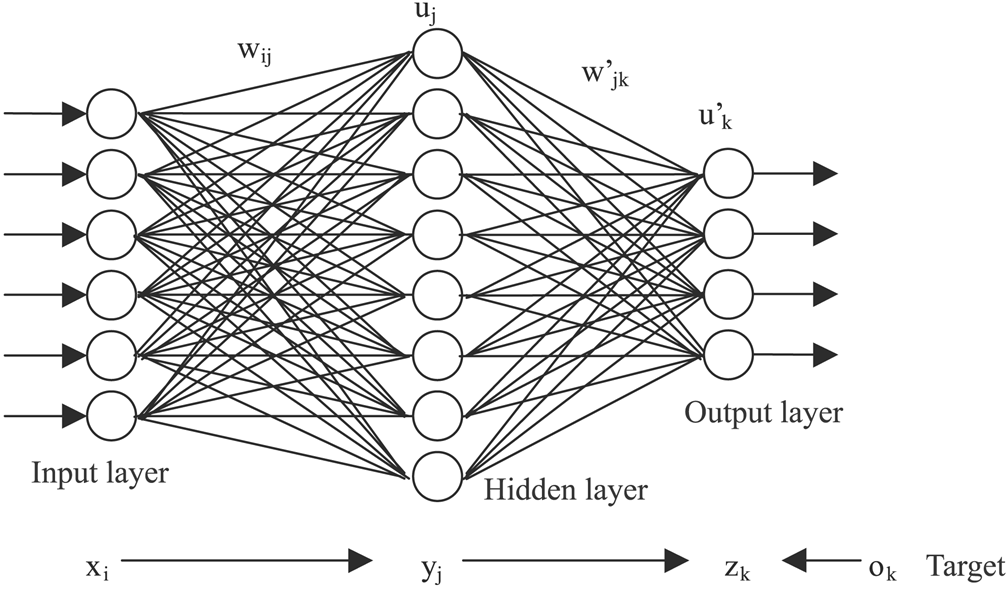
\includegraphics[width=0.7\textwidth]{neuronalesnetzwerk.png}
	\caption{Künstliches Neuronales Netzwerk\protect\cite{annpic}}
	\label{fig:Bild1}
\end{figure}
~\\\\
Jeder Layer besteht aus künstlichen Neuronen. Diese haben ihre Namensgebung von aus der Natur stammenden Neuronen, in Gehirnen von Lebewesen. Neuronen sind die Bausteine, aus denen die Gehirne von Lebewesen wie Fischen, Vögeln und Säugetieren, zusammen gesetzt sind. Neuronen, oder auch Nervenzellen, haben einen Zellkern, welcher das Zentrum der Zelle ist. Um sie herum sind Dendriten, welche die Verbindung zu anderen Neuronen her stellen. Neuronen sind untereinander mit Axonen verbunden, welche an den Enden Synapsen haben, in der eine Grenze von Axon zur Nervenzelle einen Spalt bildet. Dieser Spalt kann überwunden werden, indem von der Synapse Botenstoffe abgesendet werden, die sich dann an den Rezeptor der gegenüberliegenden Synapse anhaften. Diese Übertragung findet statt, wenn an der Synapse ein bestimmter Schwellenwert von elektrischen Reizen überschritten wurde, welchen die Zelle abfeuert lässt \cite{neuralnet}.
\\\\
Künstliche Neuronen haben diesen Schwellenwert durch sogenannte Gewichte w\textsubscript{kj} , diese sind auf den Verbindungen zwischen den Neuronen, in den unterschiedlichen Layern im KNN (vgl. \ref{fig:Bild2}). Dabei steht j für die Position im Layer und k, in welchem Layer sich das Neuron befindet.
\begin{figure}[htbp] 
	\centering
	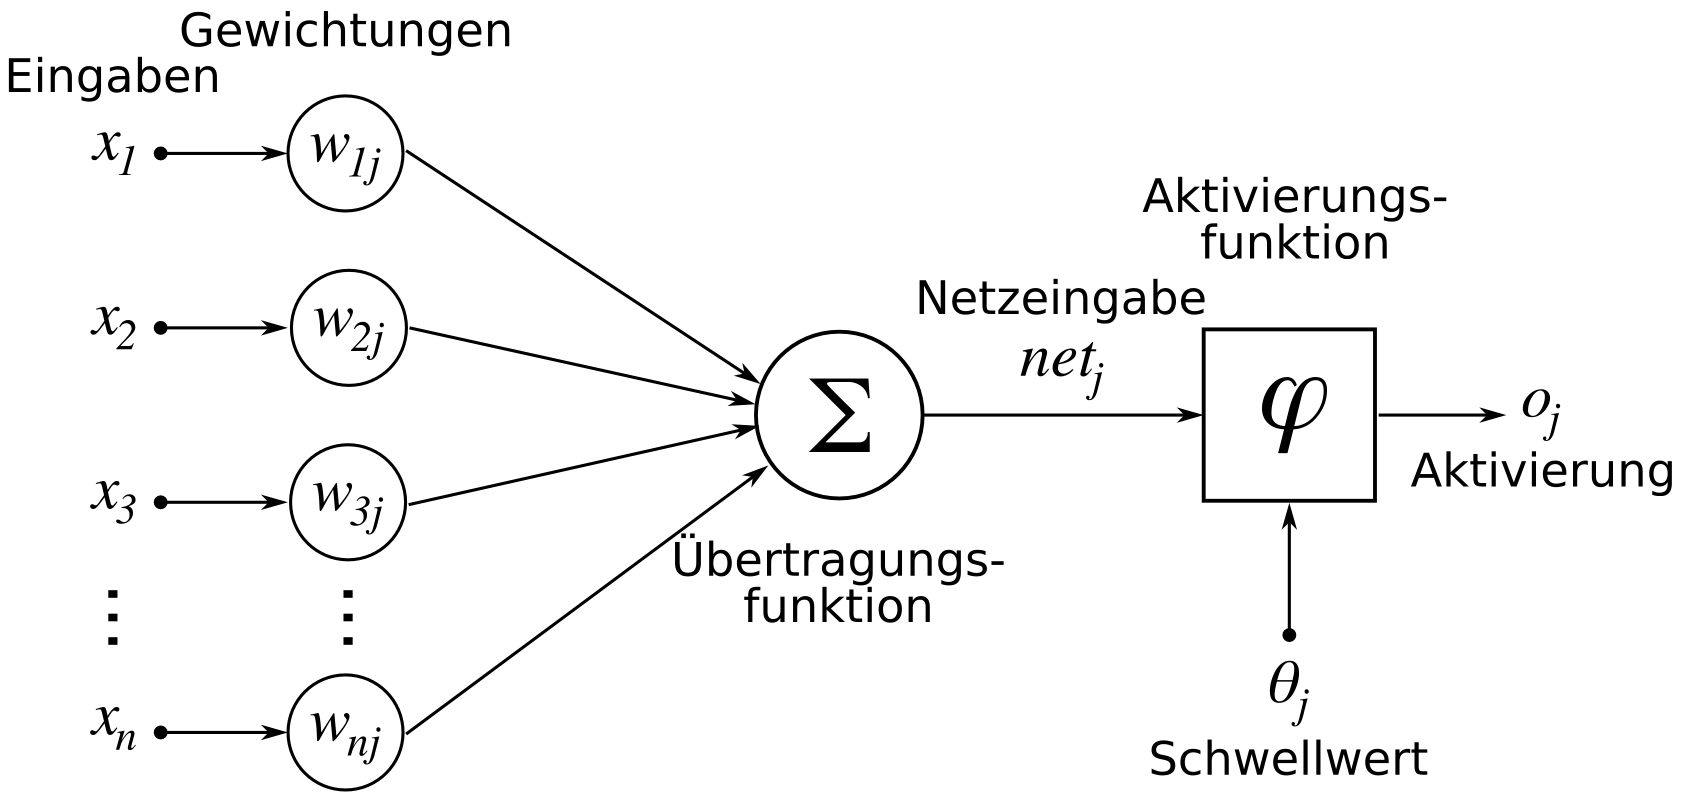
\includegraphics[width=0.7\textwidth]{Neuron.png}
	\caption{künstliches Neuron}
	\label{fig:Bild2}
\end{figure}
Jeder Layer eines KNN besteht aus mehreren Neuronen. Ein Neuron kann mehrere Inputs x\textsubscript{j} erhalten und produziert einen Output $\nu$\textsubscript{i}. Die Berechnungen, welche von den Neuron durchgeführt werden, sind zunächst jeden Input x\textsubscript{j} mit einem Gewicht w\textsubscript{ij} zu multiplizieren. Anschließend wird die Summe von x*w gebildet und ein Bias b dazu addiert. Das Ergebnis wird dann in eine Aktivierungsfunktion $\lambda$ gegeben \cite{neuralnet}. Ein Neuron ist definiert durch:
\\\\
\begin{math}
\nu\textsubscript{i} = \lambda(\sum_{j=0}^{m}(w\textsubscript{kj}+x\textsubscript{j})+b\textsubscript{k})                
\end{math}
\\\\
Die Aufgabe der Aktivierungsfunktion $\lambda$  ist es, eine nicht lineare Transformation des Inputs zu erzeugen. Damit kann das KNN nicht lineare Funktionen abbilden und somit komplexere Aufgaben lösen \cite{neuralnet}. Es gibt unterschiedliche Aktivierungsfunktionen, im Folgenden werden einige aufgezählt:
\vspace{5 mm}
\begin{description}
	\item[Sigmoid-Funktion]			
	\begin{math}
	\sigma(x)=\frac{1}{1+exp(-x)}
	\end{math}
	\vspace{5 mm}
	\item[Softmax-Funktion]	
	\begin{math}
	\zeta(x)\textsubscript{j} = \frac{e\textsuperscript{x\textsubscript{j}}}{\sum_{k=1}^{K}e\textsuperscript{x\textsubscript{k}}}
	\end{math}
	\vspace{5 mm}
	\item[Rectified Linear Unit (ReLU):]
	
	\begin{math}
	f(x)=\max(0,x) 
	\end{math}
	\vspace{5 mm}
	\item[Leacky Rectified Linear Unit(Leaky Relu):]
	
	\begin{math}
	f(x) = \begin{cases}
	x  	 & \quad \text{if } x > 0\\
	0.01x & \quad \text{sonst} 
	\end{cases}
	\end{math}
	\vspace{5 mm}
\end{description}
\vspace{5 mm}
Der Funktionsplot von Sigmoid Funktion kann Abb.\ref{fig:Bild3} entnommen werden. Dieser veranschaulichen den Wertebereich, welcher von der Aktivierungsfunktion angenommen werden kann und ihren Verlauf. 
\begin{figure}[htbp] 
	\centering
	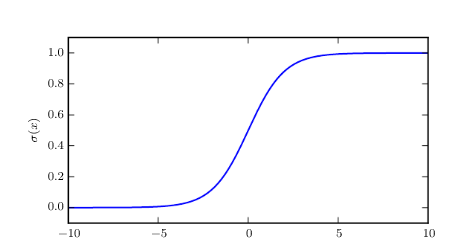
\includegraphics[width=0.5\textwidth]{sigmoid.png}
	\caption{Sigmoid Funktion}
	\label{fig:Bild3}
\end{figure}

\newpage
\subsubsection{Ziel-Funktion}\label{sec:Zielfunktion}
~\\\\
Die Ziel-Funktion J($\theta$), oder auch Loss-Funktion genannt, hat die Aufgabe zu messen, wie gut das Model $\theta$, f*(x) approximiert. Dafür wird der Begriff ''Kosten'' verwendet, wie hohe Kosten erzeugt das Model, beim Lösen der zugewiesenen Aufgabe. Die Wahl, welche Ziel-Funktion gewählt wird, ergibt sich aus der Aufgabe des KNN. Die Aufgabe kann beispielsweise einem Klassifikations- oder Regressions-Ziel entsprechen. Bei Regression soll eine kontinuierliche Variable von $\theta$ als Output generiert werden, wohingegen bei Klassifikationsproblemen der Output Klassen-Labels darstellt. Es gibt verschiedene Ziel-Funktionen, im Folgenden wird die Cross Entropy Loss Function vorgestellt. Diese kann verwendet werden um beispielsweiße Klassikationsprobleme zu lösen \cite{Grundlagen}. Sie ist definiert als:
\\\\
\begin{math}
J(\theta) =-E\textsubscript{x,y$\sim$p\textsubscript{data}}\log p\textsubscript{model}(y|x)
\end{math}
\\\\
Wobei x die Trainingsdaten bezeichnet und y die möglichen Klassen. Der Output ist die Wahrscheinlichkeit zwischen 0 und 1, ob  x\textsubscript{i} $\in$ der bestimmten Klasse enthalten ist. Auch kann sie hergenommen werden, um zu messen wie hoch die Differenz zwischen zwei Wahrscheinlichkeitsverteilungen ist.
\subsubsection{Backpropagation Algorithmus}\label{sec:test}
~\\\\
Um nun KNNs zu trainieren und den gewünschten Output y zu generieren, wird der Backpropagation Algorithmus benutzt. Dieser zählt zu den Optimierungs Algorithmen für KNN und arbeitet schneller und effizienter auf Neuronalen Netzwerken, als andere Optimierungsalgorithmen vor ihm \cite{backprob}. Das mathematisch zugrundeliegende Konzept ist ein Optimierungsproblem, der die partitielle Ableitung von  $\frac{\partial J}{\partial w}$, wobei J die Zielfunktion und w die Gewichte im zu optimierenden Neuronalen Netzwerk sind. Durch die Ermittlung der Steigung, am jeweiligen Punkt der Zielfunktion, ist man nun in der Lage zu ermitteln, in welche Richtung der Funktion die Steigung abnimmt und J dahin gehend zu optimieren. Dieses Verfahren hilft dabei, das KNN  dahingehen zu optimieren, den gewünschten Output y zu erlangen.  Anschließen kann der Loss durch die Ketten Regel aus der Differentialrechnung in die einzelnen Gewichte w\textsuperscript{ij} im Netzwerk zurück geführt werden und die Gewichte dahin gehend angepasst werden, näher an den Nullpunkt der Zielfunktion zu gelangen \cite{Grundlagen}.
\\\\
Beim Mini-batch Gradient Descent wird die Anpassung der Gewichte während des Trainings in n Batches unterteilt. Die Batches bestehen aus jeweils i Datensätzen, welche im  Trainingsdatensatz enthalten sind. Nachdem der Gradient für die i Datensätze des jeweiligen Batch berechnet wurden, werden die Gewichte $\theta$ des ANN angepasst und der nächste Batch wird zum trainieren verwendet. Solange bis e Epochen, wobei e für die Durchläufe des kompletten Trainingdatensatzes steht, passiert sind. Dieses Verfahren führt zu stabileren Trainingsergebnisse \cite{batchgradeint}.

\subsubsection{Momentum}\label{sec:momentum}
~\\\\
Momentum hat das Ziel das Gradientenverfahren des Backpropagation Algorithmus \ref{sec:test} zu beschleunigen, um ein effizienter Ergebnis herbei zu führen und ein schnelleres Lernen zu erreichen. Definiert ist dies durch:
\\\\
\begin{math}
v\textsubscript{t+1} =\mu v\textsubscript{t}-\epsilon\nabla$f$(\theta\textsubscript{t})\\\\
\theta\textsubscript{t+1}= \theta\textsubscript{t}+v\textsubscript{t+1}
\end{math}
\\\\
,wobei $\epsilon$ $>$ 0 die Lernrate ist,  $\mu$ $\in$ [0,1] das Momentum und $\nabla$f($\theta\textsubscript{t}$) der Gradient von $\theta\textsubscript{t}$. Je größer das Momentum, desto schneller bewegt sich der Gradient abwärts. Da dieser zu Beginn einer Lernphase üblicherweise hoch ist, empfiehlt es sich zunächst mit einem niedrigen Momentum zu arbeiten, da sonnst die Gefahr besteht, über das globale Optimum hinaus zu schießen. Wenn nun das Training stagniert, was auf Gründe des Aufbaus der Zielfunktion zurückzuführen ist, so dass zur Nähe des globalen Optimums flache Täler entstehen, welche das Training verlangsamen und es zu keiner Verbesserung kommt, kann man durch Momentum erzwingen, größere Gradienten Sprünge einzugehen. Und sich somit schneller zu einem globalen Optimum zu bewegen, oder aber aus einem lokalen Optimum hinaus, Richtung eines globalen Optimums, kann Momentum benutzt werden \cite{momentum}.

\subsubsection{Regularization}
~\\\\
Ein Problem, welches alle Machine Learning Anwendungen teilen, ist es wenn der Trainingsalgorithmus zunächst eine gutes Trainingsergebnis erzielt, aber dann auf dem Testdatensatz ein schlechtes Ergebnis erlangt, was Overfitting genannt wird. Ziel ist es, dass das Model generalisiert und auch Datensätze, welche nicht im Trainingsdatensatz enthalten waren, richtig klassifiziert werden. Man spricht davon, das Model zu regularizieren \cite{Grundlagen}.
~\\\\
Je mehr Daten beim Training verwendet werden, desto mehr kann generalisiert werden. Data Augmentation heißt, dass man mehr Datensätze, aus den eigentlichen Trainingsdatensatz, erstellt. Dies kann durch eine Veränderung der Trainingsdatensätze im Allgemein geschehen \cite{Grundlagen}, wenn man beispielsweise 3D-Punktwolken rotiert, um diese mehrfach zu nutzen. Eine weitere Möglichkeit ist es, bestimmte Datenpunkte in einem Datensatz zu ändern, indem man ein Objekt, welches auf einem Bild dargestellt wird, verkleinert oder vergrößert \cite{Grundlagen}.
~\\\\
\pagebreak\linebreak 
Eine weitere Möglichkeit für Regularization ist Dropout. Dabei wird während des Lernprozesses ein gewisser Prozentsatz der Neuronen in jedem Layer nicht verwendet. Dies zwingt das Netzwerk, welches sonnst die Abhängigkeiten zwischen den Neuronen lernt, eine generalisiertere Lösung zu finden \cite{dropout}.\\
~\\\\
Bei der sogenannten L2-Regularization wird das Gewicht des Neurons während des Trainings näher zu seinem Ursprung, dem Wert seiner Initialisierung, gedrängt. Dies passiert, indem ein Regularisierungswert $\Omega$ = $\frac{1}{2}||w||\frac{1}{2}$ an die Zielfunktion gehängt wird. Dies sorgt dafür, dass während des Trainings der Gewichts Vektor, welcher durch das Gradienten Verfahren ermittelt wird, schrumpft, was für eine höhere Varianz während des Trainings sorgt, was wiederum das KNN dazu zwingt, mehr zu generalisieren \cite{Grundlagen}.\\ 

\subsubsection{Batch Normalisation}
~\\\\
Dadurch, dass der Input in jedem Layer abhängig von dem vorherigen Layern ist, können Änderungen von Werten in frühen Layern des KNNs große Auswirkungen in tieferen Layern im Netzwerk haben. Dadurch resultiert, dass in Trainingsabläufen die Verteilung der Gewichte in den jeweiligen Layern verlangsamt wird. Batchnormalization soll die Werteänderung von Gewichten verringern. Dieses Problem wird auch Covariance Shift genannt. Um dies zu verhindert zeigten Sergey Ioffe und Christian Szegedy \cite{batchnorm} eine Methode, welche Batch Normalisation genannt wird. Je mehr Layer das Netzwerk hat, desto stärker ist der Covariance Shift. Der Algorithmus verändert den eigentlichen Input von Layer n zu einen normalisierten Input x des Batch normalisierten Netzwerkes \cite{batchnorm}.
\\\\
\begin{algorithm}[H]
	Input: Werte x eines Mini-Batch $B$ = \{$x\textsubscript{1},...,x\textsubscript{n}$\}\\
	\begin{math}
	\mu\textsubscript{$B$}\leftarrow\frac{1}{m}\displaystyle\sum_{i=1}^{m}$x$\textsuperscript{i}
	\end{math}\\
	\begin{math}
	\sigma\textsubscript{$B$}\leftarrow\frac{1}{m}\displaystyle\sum_{i=1}^{m}($x$\textsuperscript{i} - \mu\textsubscript{$B$})\textsuperscript{2}
	\end{math}\\
	\begin{math}
	\hat{x\textsubscript{i}}\textsubscript{$B$}\leftarrow\frac{x\textsubscript{i}-\mu\textsubscript{$B$}}{\sqrt{\sigma\textsubscript{$B$} + \epsilon}}
	\end{math}\\
	\begin{math}
	$y$\textsubscript{i}\leftarrow\gamma\hat{x\textsubscript{i}} + \beta \equiv BN\textsubscript{$\gamma$;$\beta$}($x$\textsubscript{i})
	\end{math}\\
	Output: \{$y$\textsubscript{i}=BN\textsubscript{$\gamma$;$\beta$}($x$\textsubscript{i})\}
	\caption{Batch Normalisierung angewand auf x über Input bei Mini-Batch  }	
\end{algorithm}
~\\\\
In Schritt 2 des Algorithmus 1 wird der Erwartungswert für alle Inputs von Mini-Batch B berechnet und in Schritt 3 die Varianz. In Schritt 3 wird der normalisierte x\textsubscript{i} berechnet, welche dann mit $\beta$ und $\gamma$ multipliziert werden. Diese Werte sind neue Gewichte im Neuronalen Netzwerk, welche während des Trainingsprozesses angepasst werden. $\epsilon$ in der Gleichung in Zeile 4 ist nur dafür da, damit nicht durch 0 geteilt werden kann \cite{batchnorm}. In Abb. \ref{fig:Bild6} ist veranschaulicht, wie die Batch-Normalization-Layer in das KNN eingebaut werden. 

\begin{figure}[htbp] 
	\centering
	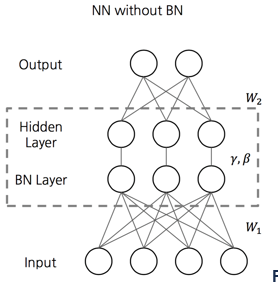
\includegraphics[width=0.5\textwidth]{batchnorm.png}
	\caption{Neuronales Netzwerk mit Batch-Normalization-Layer\protect\cite{batchnormweb}}
	\label{fig:Bild6}
\end{figure}
\subsection{Convolutional Neural Networks}

Convolutional Neural Networks (CNN) sind eine spezielle Art von künstlichen neuronalen Netzwerken. Sie sind dafür konzipiert auf Datensätzen zu arbeiten, welche in eine Matrix Form gebracht worden sind. Der Input eines CNN können beispielsweise Bilder sein, welche durch die Matrix A =
$
\begin{bmatrix}
a_1	& a_1	& \dots	 & a_n     \\
b_1	& b_2 	& \dots  & b_n	  \\
\vdots	& n_n 	& \ddots & \vdots \\
x_1 	& x_2 & x_3	 & x_n
\end{bmatrix}
$
\\\\dargestellt werden \cite{Grundlagen}. Jedes Element x\textsubscript{ij} stellt einen Pixel eines Bildes dar, wobei x\textsubscript{n} $\in$ [0,255] . Die Matrix A\textsuperscript{w$\cdot$b$\cdot$c} stellt w$\cdot$b$\cdot$c = N dimensionale Matrix dar. Wobei w der Länge und b Breite des Bildes entspricht. c sind die Farbspektren eines Bildes, diese sind in einem RGB-Farbraum 3, beziehungsweise in einem schwarz-weiß Bild 1. Nachdem  der Input eines CNN definiert ist, kommt nun der Aufbau. CNN setzen sich aus mehrere Schichten von Convolution Layern zusammen. Ein Netzwerk kann mehrere N-Layer haben, wobei jeder Layer aus mehreren Convolutions, oder auch Kernels genannt, zusammengesetzt ist. Ein Aufbau kann Abb. \ref{fig:Bild10} entnommen werden.
\begin{figure}[htbp] 
	\centering
	\includegraphics[width=0.9\textwidth]{convol.png}
	\caption{Convolutional Neural Network}
	\label{fig:Bild10}
\end{figure}
Die Kernels, also die einzelnen Filter, von denen jeder N-Layer k besitzt, sind K\textsuperscript{n$\cdot$n} Matrizen. Jedes k\textsubscript{ij} in einem Filter einspricht einem, aus der üblichen Neuronalen Netzwerk Architektur bekanntem Gewicht. Diese Gewichte werden dann durch den Backpropagation-Algorithmus in der Trainingsphase des Netzwerkes angepasst, um den Verlust der Ziel-Funktion durch das Bestimmen des Gradienten zu minimieren \cite{Grundlagen}. Das in Abb. \ref{fig:Bild10} dargestellte Subsampling ist der Output aus den Convolutional Layern. 
\\\\
Da Input und Kernel unterschiedliche Größen haben und man den gesamten Input mit dem Kernel abdecken möchte, bewegt sich der Filter um s Position auf den Input und führt erneut einen Berechnungschritt durch. Dieser Vorgang wird Stride genannt. An jeder Position wird das Produkt von jedem x\textsubscript{ij} des Inputs und k\textsubscript{ij} des Kernels durchgeführt.  Anschließend werden alle Produkte aufsummiert. In Abb. \ref{fig:Bild11} ist dieser Vorgang verdeutlicht. Zusätzlich gibt es die Möglichkeit für das sogenannte Zero Padding P. Dabei werden mehrere 0 um die Input Feature Map, am Anfang und Ende der Axen, anfügt. Dies ist notwendig, wenn die Kernel und Input Größen nicht kompatible zueinander sind. Die Anzahl der möglichen Positionen ergibt sich aus der Kernel Größe und dem Input des jeweiligen Kernels, sowie des Strides. Die Output Größ W kann durch W = (W-F+2P)/s+1 berechnet werden, wobei F für die Größe des Kernels steht \cite{conv}.
\pagebreak\linebreak 
\begin{figure}
	\centering
	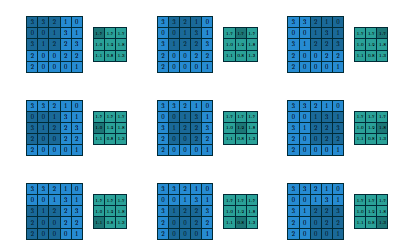
\includegraphics[width=0.7\textwidth]{conv.png}
	\caption{Convolution Beispiel\protect\cite{conv}}
	\label{fig:Bild11}
\end{figure}
Um  besser zu verstehen, welche Auswirkungen die Anzahl der Kernels in Layer n auf die Größe des Outputs von n und die Anzahl der Kernels in Layer n+1 für den nächsten Layer haben, wird ein Beispiel aufgezeigt. Der erste Layer hat 20 Kernels mit der Größe 7x7 und Stride 1. Der Input A für einen Kernel K ist eine 28x28 Matrix. Der Output aus diesen Filter sind 20 22x22 Feature Maps. Wäre der Input ein 28x28x3 Bild, mit 3 RGB Channels, wäre der Output 60 22x22 Feature Maps. Allgemein kann Convolution Layer als Subsampling gesehen werden und Stride gibt an, wie viele Dimensionen bei diesem Prozess pro Convolution Layer entfernt werden soll. Der letzte Layer ist ein Fully-Connected Layer, welcher den typischen Anforderungen von ANN entspricht \cite{conv}.  
\\\\
Transposed Convolution, auch genannt Fractionally Strided Convolution oder Deconvolution, ist eine Umkehrfunktion von der üblichen Convolution. Es verwendet die gleichen Variablen wie Convolution. Dabei wird ein Kernel K mit der Größe N x N definiert, der Input I mit der Größe N x N und Stride s = 1. Deconvolution kann wie Convolution angesehen werden, mit  Zero Padding auf dem Input.  Das in Abb. \ref{fig:Bild12} gezeigte Beispiel zeigt einen deconvolution Vorgang mit einem 3x3 Kernel über einem 4x4 Input. Dies ist gleich zusetzten mit einem Convolution Schritt, mit einem 3x3 Kernel auf einem 2x2 Input und einer 2x2 Zero Padding Grenze. Convolution ist Supsampling und mit Deconvolution wird Upsampling betrieben. Durch diesen Schritt kommt es zu einer Dimensionserhöhung des Inputs. Die Gewichte der Kernels bestimmen wie der Input transformiert wird. Durch mehrere Schichten von Deconvolution Layer kann von einer Input Größe NxN auf eine Output Größe KxK gekommen werden, wobei K $>$ N mit Abhängigkeit von Kernel und Stride abgebildet werden\cite{conv}. 

\begin{figure}[htbp] 
	\centering
	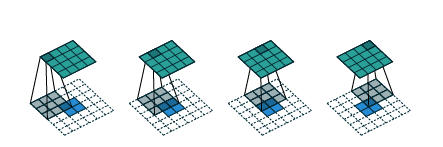
\includegraphics[width=1.0\textwidth]{decon.png}
	\caption{Deconvolution Beispiel \protect\cite{conv}}
	\label{fig:Bild12}
\end{figure}
\newpage
\subsection{Autoencoder}\label{sec:autoencoder}

Autoencoder gehören zu den generativen Modellen im Bereich des Machine Learnings. Generative Modelle haben das Ziel eine Wahrscheinlichkeitsverteilungen von Daten zu erlernen. Anschließend kann diese als ein Modell genutzt werden, um Samples aus dieser zu erzeugen. Die Modelle können dabei beispielsweise auf KNN oder Markov Chains trainiert werden. Im Folgenden liegt der Fokus auf KNNs. Allgemein gehalten können jegliche Typen von Daten wie Text, Bild oder Audiodateien, für generative Modelle herangezogen werden. Es gibt unterschiedliche Typen von generativen Modellen, welche sich vom Aufbau des Neuronalen Netzwerk und der Zielfunktion unterscheiden. Beispiele dafür sind Boltzmann Maschine, Autoencoder oder Deep Belief Networks \cite{Grundlagen}. 
\\\\
Autoencoder sind eine andere Art von Model aus dem Bereich der generativen Modelle. Ihre Aufgabe besteht darin, einen Input zu komprimieren und aus der komprimierten Information den Input wieder herzustellen. Die Technik, auf welche Autoencoder zurückgreifen, nennt sich Dimensionreduktion. Dabei wird die Dimension der Daten so reduziert, dass nur Informationen bei behalten werden, welche als relevant gelten. Diese Technik findet auch in anderen Machine Learning Modellen Anwendung, wie beispielsweise bei der Principale component anaysis(PCA) Anwendung \cite{dimreduction}.  Ein Autoencoder besteht aus 2 Bestandteilen. Erstens einem Encoder e, dargestellt als z=$f$(x), welcher einen Input x $\in$ von $x\textsuperscript{i}$, wo x ein Vektor der Länge i ist und damit die Input Dimension bestimmt. Dieser wird durch den Encoder auf einem Vektor $z\textsuperscript{k}$ abgebildet, wobei k$<$i ist. Zweitens der Decoder d, dargestellt als x`=g(z), dieser bekommt als Input $z\textsuperscript{k}$ und bildet z auf $r\textsuperscript{l}$ ab, wobei l = i und somit die gleiche Dimension wie der Input. Die Aufgabe ist es nun, dass der Encoder den Input x so gut komprimiert, dass der Decoder es schafft, das x $\thickapprox$ x` ist \cite{Grundlagen}. Eine grafische Darstellung kann aus Abb. $\ref{fig:Bild13}$ entnommen werden. 
\\\\
Der Autoencoder wird durch den in Kapitel \ref{sec:test} vorgestellten Algorithmus trainiert und erlernt so beispielsweise durch Fully-Connected-Layer,  Convolutional-Layer oder Deconvolutional-Layer. Eine Metrik um zu messen wie das Modell seine Aufgabe erfüllt, könnte beispielsweiße die Cross-Entropy-Funktionen sein, welche schon in Kapitel \ref{sec:Zielfunktion} vorgestellt worden ist. Weitere spezifische Zielfunktionen für Autoencoder, welche mit 3D Punktwolken arbeiten und für die folgende Arbeit von belangen sind, werden nun vorgestellt.
\begin{figure}[htbp] 
	\centering
	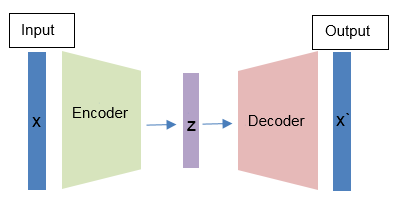
\includegraphics[width=1.0\textwidth]{autoencoder2.png}
	\caption{Autoencoder}
	\label{fig:Bild13}
\end{figure}
Bei Punktwolken als Datentyp erzielt die Cross-Entropy-Funktion keine guten Ergebnisse, da diese invariant zu ihrer Permutation sind. Da dieser Arbeit der Input von 3D Pointclouds zugrunde liegt und diese Sets  invariant zu ihren Permutationen sind. Ändert sich die Anordnung der einzelnen Punkte im Set, bleibt das dargestellte Ergebnis unverändert.  Deshalb kann nicht auf übliche Zielfunktionen, welche für strukturierte Daten wie Bilder verwendet werden, zurück gegriffen. Die Herausforderung besteht darin, zwischen zwei unterschiedliche Sets von Punkten heraus zu finden, wie hoch die Diskrepanz zwischen den beiden Sets ist \cite{invariant}. 
\\\\
Eine Möglichkeit, speziell für Autoencoder, welche mit Punktwolken arbeiten, ist die Earth Mover Distance (EMD). Bei dieser sind X\textsubscript{1} und X\textsubscript{2} zwei Punktwolken, mit jeweils x\textsubscript{n} definierten Punkten \cite{autoencoderloss}. Definiert ist sie durch die Funktion:
\\\\
\begin{math}
d\textsubscript{EMD}=\min_{\theta : X\textsubscript{1}\rightarrow X\textsubscript{2}}  \sum_{x\in X\textsubscript{1}}|| x - \theta(x)||\textsubscript{2};wobei\;\theta: X\textsubscript{1} \rightarrow X\textsubscript{2}\, bijektiv\, ist 
\end{math}
\\\\
Grafisch kann man die Berechnung wie in Abb. \ref{fig:Bild14} darstellen. Ein Punkt von x\textsubscript{n} $\in$ X\textsubscript{1} wird dem nächsten Punkt y\textsubscript{n} $\in$  X\textsubscript{2} zugewiesen. Wobei die Distanz durch die Euklidische Distanz der jeweiligen Punkte ermittelt wird. 
\begin{figure}[htbp] 
	\centering
	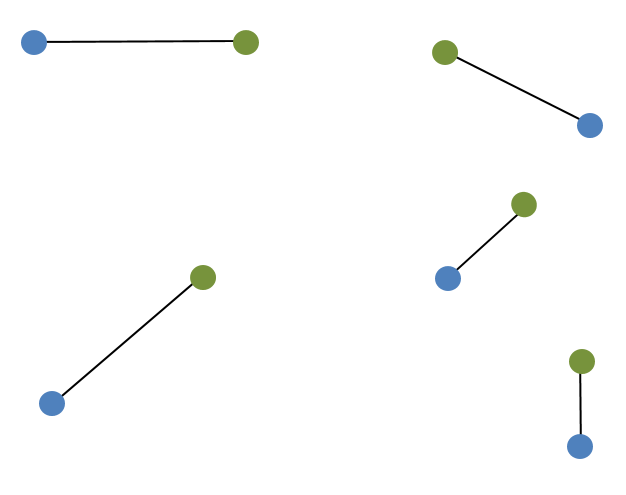
\includegraphics[width=0.5\textwidth]{emd_distance.png}
	\caption{Earth Mover Distance für Punktwolken \protect\cite{3dpointcloud}}
	\label{fig:Bild14}
\end{figure}		
Eine weitere Möglichkeit ist die Chamfer Distance (CD). Wie auch zuvor sind  X\textsubscript{1} und X\textsubscript{2} zwei Punktwolken, mit jeweils x\textsubscript{n} definierten Punkten \cite{autoencoderloss}. Definiert ist sie durch die Funktion:
\\\\
\begin{math}
d\textsubscript{CD}(X\textsubscript{1},X\textsubscript{2})=\sum_{x\in X\textsubscript{1}} \min_{y \in X\textsubscript{2}}||x-y|| + \sum_{y\in X\textsubscript{2}} \min_{x \in X\textsubscript{2}}||x-y||
\end{math}
\\\\
Der Unterschied ergibt sich zwischen den beiden Metriken, so dass bei der EMD der Ausgangswolke die Punkte zu der anderen jeweils optimiert werden. Wohingegen bei der CD die Distanzen von und zu der Ausgangspunktwolke berechnet wird. Dies geht aus Abb. \ref{fig:Bild15} hervor, in welcher die Distanzberechnung der einzelnen Punkte dargestellt wird \cite{autoencoderloss}.
\begin{figure}[htbp] 
	\centering
	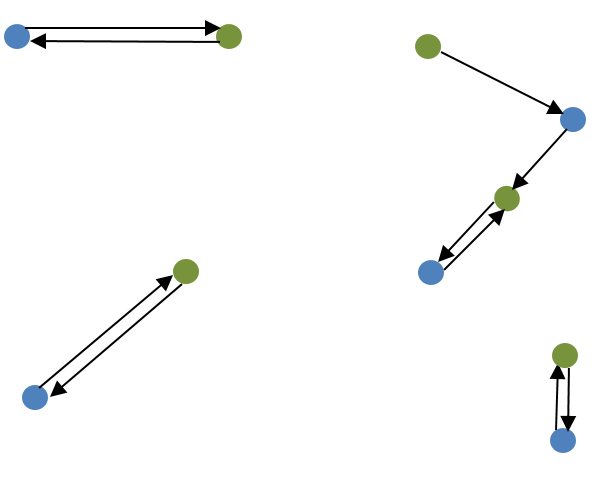
\includegraphics[width=0.5\textwidth]{champfer.png}
	\caption{Chamfer Distance für Punktwolken \protect\cite{3dpointcloud}}
	\label{fig:Bild15}
\end{figure} 
\newpage
\subsection{Generative Adversarial Network}

Ein GAN besteht aus zwei KNN, dem Discriminator D und dem Generator G. Das Ziel des G ist es, Daten x zu erzeugen, welche nicht von Trainingsdaten y unterschieden werden können. Dabei wird eine vorangegangene Input Noise Variable p\textsubscript{z}(z) verwendet, welche eine Abbildung zum Datenraum G(z;$\Phi$\textsubscript{g}) herstellt. Dabei sind $\Phi$\textsubscript{g} die Gewichte des neuronalen Netzwerkes von G. Der Discriminator hat die Aufgabe zu unterscheiden, ob der jeweilige Datensatz von G erzeugt wurde und somit ein fake Datensatz ist, oder von Trainingsdaten y stammt \cite{goodfellow2014}. Die Zusammensetzung zwischen den beiden Netzwerken kann aus Abb. \ref{fig:Bild20} entnommen werden.
\\
\begin{figure}[htbp] 
	\centering
	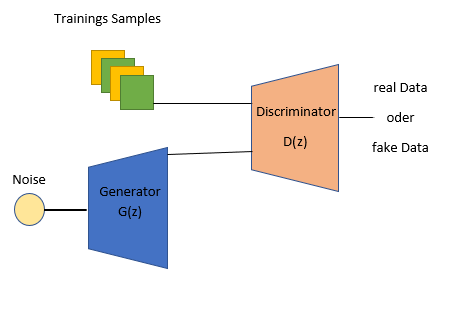
\includegraphics[width=0.5\textwidth]{GAN_GRUNDAUFBAU.png}
	\caption{Generativ Adversarial Network \protect\cite{ganpic}}
	\label{fig:Bild20}
\end{figure}
\\
Der Discriminator ist definiert durch D(x;$\Phi$\textsubscript{d}). Wobei $\Phi$\textsubscript{d} die Gewichte des Discriminators sind und D(x) die Wahrscheinlichkeit ist, dass x von den Trainingsdaten stammt und nicht von p\textsubscript{g}. Die Wahrscheinlichkeitsverteilung für unsere Trainingsdaten ist p\textsubscript{r}.  Im Training werden dann $\Phi$\textsubscript{d} so angepasst, dass die Wahrscheinlichkeit Trainingsbeispiele richtig zu klassifizieren maximiert wird. $\Phi$\textsubscript{g} wird dahingehen trainiert, die Wahrscheinlichkeit zu minimieren, so dass D erkennt, dass Trainingsdatensatz x von G erzeugt wurde. Mathematisch ausgedrückt durch log(1 - D(G(z))). Die gesamte Loss-Funktion des Vanilla GAN ist definiert als:
\\\\
\begin{math}
min\textsubscript{G} max\textsubscript{D}V(D,G)=E\textsubscript{x$\sim$p\textsubscript{data}(x)}[logD(x)]  + E\textsubscript{z$\sim$p\textsubscript{z}(z)}[log(1-D(G(z))]
\\\\             
\end{math}
Diese beschreibt ein Minmax Spiel zwischen G und D, welches das globale Optimum erreicht hat wenn p\textsubscript{g} = p\textsubscript{r}. Das heißt, wenn die Datenverteilung, welche von G erzeugt wird, gleich der unserer Trainingsdaten ist \cite{goodfellow2014}. 
\pagebreak\linebreak
Das Training erfolgt durch den folgenden Algorithmus  \cite{goodfellow2014}:
\\
\begin{algorithm}[H]
	\For{Anzahl von Training Iterationen}{\For{k Schritte}{$\bullet$Sample minibatch von m noise  Samples z\textsuperscript{(1)},...,z\textsuperscript{(m)}von noise p\textsubscript{g}(z)\\
	$\bullet$ Sample minibatch von m Beispielen x\textsuperscript{(1)},...,x\textsuperscript{(m)}von Daten Generationsverteilung p\textsubscript{data}(x)\\
    $\bullet$ Update den Discriminator zum aufsteigenden stochastischen Gradienten:\\
\begin{math}
\nabla\textsubscript{$\Phi$\textsubscript{d}}\frac{1}{m}\sum_{i=1}^{m}[logD(x\textsuperscript{(i)})+log(1-D(G(z\textsuperscript{(i)})))]
 \end{math}

}$\bullet$ Sample minibatch von m noise Samples z\textsuperscript{(1)},...,z\textsuperscript{(m)} von noise p\textsubscript{g}(z)\\$\bullet$ Update den Generator mit den absteigenden stochastischen Gradienten: \\\begin{math} 
\nabla\textsubscript{$\Phi$\textsubscript{g}}\frac{1}{m}\sum_{i=1}^{m}log(1-D(G(z\textsuperscript{(i)})))\end{math}}
		\caption{Minibatch stochastic gradient descent Training für Generative Adversarial Networks. Die Anzahl der Schritte welche auf den Discriminator angewendet wird ist k }	
\end{algorithm}
~\\
Beim Training wird ein stochastischer Minibatch von mehren Trainingsdaten gleichzeitig erstellt. Dies soll dabei helfen, dass der Generator sich nicht auf bestimmte Gewichte fest fährt und auf Trainingssätze kollabiert. So weisen die erzeugten Daten mehr Variationen auf \cite{improvingan}. D wird zunächst in einer inneren Schleife auf n Trainingsätzen trainiert, womit man Overfitting von D vermeiden will, was zur Folge hätte, dass D nur den Trainingsdatensatz kopieren würde. Deshalb wird k mal D optimiert und ein mal G in der äußeren Schleife  \cite{goodfellow2014}. 
\\\\
Ein möglicher Aufbau von GAN wird in Abb. \ref{fig:Bild21} dargestellt. Dies ist das sogenannte Deep Convolution GAN(DC GAN), welches dafür konzipiert wurde auf Bilddaten zu arbeiten. Dabei besteht der Generator aus mehren Schichten von Deconvolutional-Layern, welcher den Input Noise Variable p\textsubscript{z}(z) auf y abbildet. D besteht aus mehren Schichten von Convolutional-Layern und bekommt als Input die Trainingsdaten, oder die von G erzeugten Y, und entscheidet über die Klassifikation \cite{dcgan}.
\begin{figure}[htbp] 
	\centering
	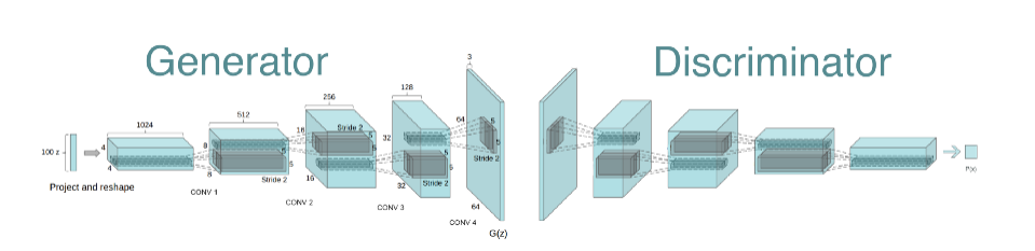
\includegraphics[width=1.0\textwidth]{dcgan1.png}
	\caption{Deep Convolutional GAN\protect\cite{dc-gan_book}}
	\label{fig:Bild21}
\end{figure}
Goodfellow \cite{goodfellow2014} zeigte, dass sich die MinMax Loss-Funktion des GAN auch als Jensen-Shannon Divergenz(JS Divergenz) darstellen lässt. Diese ist definiert als:
\\\\
\begin{math} D\textsubscript{JS}(P\textsubscript{r}|| P\textsubscript{g}])=\frac{1}{2}D\textsubscript{KL}(P\textsubscript{r}|| \frac{P\textsubscript{g}+P\textsubscript{r}}{2}])+D\textsubscript{KL}(P\textsubscript{q}|| \frac{P\textsubscript{g}+P\textsubscript{r}}{2}])  
\end{math}
\\\\
wobei P\textsubscript{r} die Wahrscheinlichkeitsverteilung der Trainingsdaten ist und P\textsubscript{g} die des Generators. Huzár \cite{sha} zeigte, dass durch das symmetrische Verhalten der JS Divergenz ein potentiell besseres Trainingsergebnis entstehen kann, im Vergleich zu der Kulbach Leibler Divergenz, welche von anderen generativen Modellen, wie Autoencoder, verwendet wird. Damit zeigte er, weshalb GANs im Vorteil gegenüber anderen generativen Modellen sind.
\subsubsection{Probleme mit GANs}\label{sec:problemegan}
~\\\\
Wie auch andere generative Modelle, haben GANs noch Schwächen bezüglich der Trainingsabläufe und der Qualität ihrer generierten Daten. Im Folgenden wird auf einige Probleme eingegangen, für welche im darauffolgenden Kapitel Lösungsansätze aufgezeigt werden. 
~\\\\
Der Vanishing Gradient beschreibt das Problem, wenn D perfekt trainiert ist, weil die beiden Datenverteilungen p\textsubscript{r} und p\textsubscript{g} disjunkt sind und es keine Überlapp-ung der Datenverteilungen gibt. Die Loss-Funktion würde in diesem Fall auf 0 fallen und es gäbe keinen Gradienten, für den die Gewichte von G angepasst werden können. Dies verlangsamt den Trainingsprozess, bis hin zu einem kompletten Stopp des Trainings. Würde D zu schlecht trainieren, mit D(x) = 0 für p\textsubscript{r} und  D(x) = 1 für p\textsubscript{g}, bekommt G kein Feedback über seine Leistung bei der Datengeneration und hat keine Möglichkeit p\textsubscript{r} zu erlernen \cite{vanishing}.
~\\\\
Ein weiteres Problem kann das sogenannte Equilibrium hervorrufen. In diesem Fall betreiben D und G ein MinMax Spiel. Beide versuchen das Nash Equilibrium zu finden. Dies ist der bestmögliche Endpunkt in einem nicht kooperativen Spiel. Wie in dem Fall von GAN wäre dies wenn  p\textsubscript{g} = p\textsubscript{r}. Es wurde gezeigt, dass das Erreichen dieses Punktes sehr schwierig ist, da durch die Updates der Gewichte mit den Gradienten der Loss-Funktion starke Schwingungen der Funktion entstehen können. Dies kann zu einem instabilen Orbit für das laufende Training führen \cite{improvingan}.   
~\\\\
Abschließend sei noch der Mode Collapse zu erwähnen. Dieses Problem entsteht, wenn der Generator während des Trainings an einem bestimmten Setting seiner Gewichte festhält und er bei der Datengeneration sehr ähnlichen Samples generiert \cite{improvingan}.

\subsubsection{Lösungsansätze für die GAN Probleme}
~\\\\
Im folgenden werden einige Techniken aufgezeigt, welche die unter dem Abschnitt ''Probleme mit GAN'' genannten Schwierigkeiten angehen und zu einem effizienteren Training führen, damit eine schnellere Konvergenz während des Trainings erreicht wird.
~\\\\
Um das Problem des Mode Collapse zu umgehen, kann Minibatch Discrimination angewendet werden. Damit es nicht zu einem Festfahren der Gewichten von G kommt, wird beim Trainieren die Nähe der Trainingsdatenpunkten gemessen. Anschließend wird die Summe über der Differenz aller Trainingspunkte genommen und dem Discriminator als zusätzlicher Input beim Training hinzugegeben \cite{improvingan}.\\
~\\\\
Beim Historical Averaging werden beim Training die Gewichte von G und D aufgezeichnet und je Trainingsschritt verglichen. Anschließend wird an die Loss-Funktion je Trainingschritt die Veränderung zu dem vorherigen Trainingschritt addiert. Damit soll verhindert werden, dass das Model sich zu sehr von seinem vorherigen Zustand der Gewichte entfernt \cite{improvingan}.\\
~\\\\
Eine weitere Möglichkeit ist das One-sided Label Smoothing. Hierbei werden die üblichen Label für den Trainingsdurchlauf von 1 und 0 durch die Werte 0.9 und 0.1 ersetzt. Dies führt zu besseren Trainingsergebnissen. Es gibt derzeit lediglich empirische Belege für den Erfolg, jedoch keine, weshalb diese Technik besser funktioniert \cite{improvingan}.\\
~\\\\
Der erfolgversprechendste Lösungsansatz ist die Wasserstein Metrik, oder auch Earth Mover Distance (EMD) genannt. Diese misst die Minimum Kosten, welche entstehen wenn man Daten von der Datenverteilungp p\textsubscript{r} zur Datenverteilung p\textsubscript{g} überträgt. Es wird oft auch von ``Masse`` oder ``Fläche`` gesprochen, welche von p\textsubscript{r} zu p\textsubscript{g} getragen wird. Definiert ist sie durch:
\\\\
\begin{math} 
$
W(p\textsubscript{r},p\textsubscript{g})=$\inf_{\gamma\in\prod(P\textsubscript{r},P\textsubscript{g})}$E\textsubscript{(x,y)$\sim\gamma$}[$\parallel$x - y$\parallel$]
$
\end{math}
\\\\
p\textsubscript{r} steht für die reale Datenverteilung, welche uns Daten im Form von Trainingsdaten zur Verfügung stellt und p\textsubscript{g} steht für die generierte Datenverteilung, welche von einem Model erzeugt wird. Dabei wird nun das Infinum von allen möglichen Transportplänen $\gamma$ ausgewählt, welche in $\prod$ enthalten sind, was der kostengünstigste Plan ist, die Daten von x zu y zu übertragen. Die EMD sind nun die Kosten von einem optimalen Transportplan. Vorteile sind unter anderem, dass der Gradient gleichmäßiger ist und das WGAN besser lernt, auch wenn der Generator  im Vergleich zum üblichen GAN schlechtere Daten erzeugt \cite{wasser}. Durch die Kantorovich-Rubinstein Methode kann die Wasserstein-Distanz umgeformt werden zu:
\\\\
\begin{math} 
$
$\max$\textsubscript{w$\in$W}E\textsubscript{x$\sim$P\textsubscript{r}}[f\textsubscript{w}(x)]-E\textsubscript{z$\sim$P\textsubscript{z}}[f\textsubscript{w}(g\textsubscript{$\theta$}(z))]
$
\end{math}
\\\\
Durch diese Umformung und den Verlust von Infinium bei den Transportplänen, ist es nun möglich, dass GAN die EMD nutzt, um die von G generierten Daten mit den realen Daten zu vergleichen. Dabei übernimmt der Discriminator nun die Aufgabe eines Critic, welcher nun nicht mehr 0 oder 1 für Fake oder Real ausgibt sondern einen Score, welcher angibt wie viel Masse von  g\textsubscript{$\theta$}, also dem Generator, umverteilt werden muss, damit dieser bessere Ergebnisse liefert. Das Wasserstein GAN liefert bis dahin die erfolgreichste Verbesserung zum üblichen Vanilla-GAN von Goodfellow und erlaubt es, gegen die in Kapitel \ref{sec:problemegan} aufgezeigten Probleme Vanishing gradient und Model Collapse anzugehen \cite{wasser}. 
\newpage
\subsection{Conditional-GAN}\label{sec:cgan}

Conditional-GAN(C-GAN) ist eine Modifikation des ursprünglichen GAN von Goodfellow, welche es erlaubt, bedingte Wahrscheinlichkeiten in Datensätzen zu erlernen und zusätzliche Informationen in den Lernprozess einzuspeisen, um den Output zu modifizieren. Im ursprünglichen GAN gibt es keine Möglichkeit auf den Output des Generators Einfluss zu nehmen. Das Modell wird verändert indem eine zusätzliche Information y als Input in den Discriminator und Generator eingefügt wird. Dabei kann y jegliche Information, sein wie beispielsweise Label, Bilddaten oder 3D-Daten. Dementsprechend muss die Zielfunktion dahingehend angepasst werden, bedingte Wahrscheinlichkeiten zu erlernen \cite{cgan}. 
\\\\
\begin{math}
min\textsubscript{G} max\textsubscript{D}V(D,G)=E\textsubscript{x$\sim$p\textsubscript{data}(x)}[logD(x|y)]  + E\textsubscript{z$\sim$p\textsubscript{z}(z)}[log(1-D(G(z|y))]          
\end{math}
\\\\
\begin{figure}[htbp] 
	\centering
	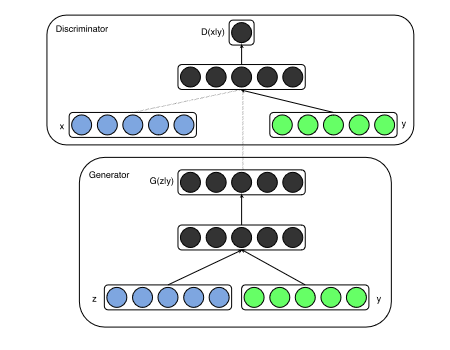
\includegraphics[width=0.5\textwidth]{cgan.png}
	\caption{Conditional Adverserial Network\protect\cite{cgan}}
	\label{fig:Bild38}
\end{figure}
\\\\
Auf Abb. \ref{fig:Bild38} kann der Informationsfluss und die Konnektivät der einzelnen Module entnommen werden. Die Module Generator und Discriminator bleiben gleich und können von ihrem Aufbau für die jeweiligen Datentypen verändert werden und so beispielsweise aus Convolutional-Layer, Deconvolutional-Layer oder Fully-Connected-Layer bestehen.
\newpage
\subsection{3D-GAN}\label{sec:3dgan}

Das Besondere am 3D Raum, im Vergleich zu normalen 2D Bildern, ist die Steigerung der Dimension und zugleich der hohe Informationsgehalt, welcher in 3D Objekten steckt. Das Ziel von 3D-GAN ist es, die Datenverteilung der zugrundeliegenden 3D-Modelle zu erlernen. Dabei wird der latente Objektraum erfasst und soll dadurch die Wahrscheinlichkeiten für einzelne Objektklassen enthalten. 
\\\\
Es wurden bereits mehrere Versuche von generativen Modellen auf 3D Daten durchgeführt, wie von Wu, Jiajun und Zhang \cite{3d}, die in ihrem Modell mit 3D-Voxel Daten arbeiten und damit ein GAN trainiert haben. Oder auch Achlioptas, Panos und Diamanti\cite{3dgan}, die ein GAN auf Punktwolken trainiert haben. Da in folgender Arbeit die 3D-Daten durch Punktwolken dargestellt werden, wird das Herangehen von Achlioptas, Panos und Diamanti näher beleuchtet.
\\\\
Die Architektur des typischen 3D-GAN, oder auch RAW-GAN genannt, ist dem Vanilla GAN von Goodfellow ähnlich. Der Input Layer ist ein Fully-Connected Layer, welcher der Anzahl der Punkte je Punktwolke * 3 entspricht. Dieser bekommt als Input einen Noise-Vektor, welcher einer Normal Verteilung entnommen und durch mehrere Layer gereicht wird, bis hin zum Output Layer, welche aus der Anzahl der gewünschten Punkte besteht. Als Zielfunktion kann mit der Vanilla-GAN-Zielfunktion oder der Wasserstein Metrik gearbeitet werden, welche im Versuchsaufbau von Achlioptas, Panos und Diamanti besser Ergebnissee geliefert hat. Der Aufbau unterscheidet sich nicht von Vanilla-GAN \cite{3dgan}. 
\begin{figure}[htbp] 
	\centering
	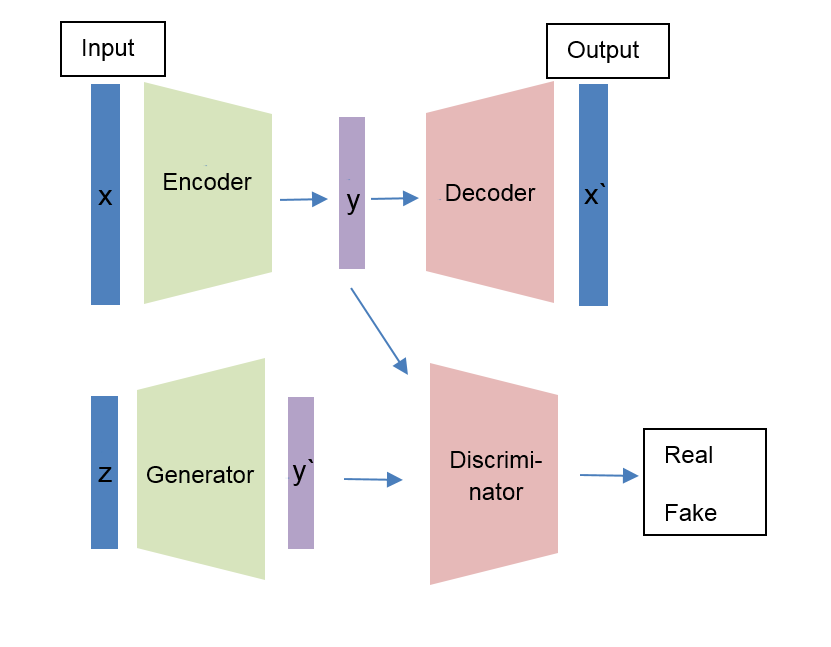
\includegraphics[width=0.5\textwidth]{latentgan.png}
	\caption{Latent-GAN}
	\label{fig:Bild39}
\end{figure}
~\\\\
Eine weitere Möglichkeit ist das Latent-GAN, dieses benutzt einen andere Aufbau, verglichen mit dem RAW-GAN, welches dabei helfen soll den latenten Raum der Objekte zu erlernen. Zunächst wird ein Autoencoder mit den vorhanden Trainingsdaten (vgl. \ref{sec:autoencoder}) trainiert. Der Aufbau ist derselbe, wie bei einem üblichen 3D-Autoencoder unter Kapitel \ref{sec:autoencoder} beschrieben. Das Ziel ist es, den latenten Raum der Trainingsdaten zu erlernen und eine Kompression der Daten um den Suchraum, der beim RAW-GAN durch die Inputdimension gegeben ist, zu verringern und dadurch das Training des GANs zu erleichtern \cite{3dgan}. 
\\\\
Bevor das Training des Latent-GAN beginnen kann, werden die Trainingsdaten durch den vorher trainierten Encoder des 3D-Autoencoder auf die festgelegte Output-Dimension komprimiert. Anschließend werden diese komprimierten Daten verwendet, um das GAN zu trainierten. Dabei erlernt das GAN komprimierten Code zu produzieren, welcher anschließend durch den Decoder des 3D-Autoencoder wieder auf die ursprüngliche Größe gebracht werden kann. Durch dieses Verfahren ist es möglich, Daten in einer guten Qualität zu produzieren und die Datenverteilung des zugrundeliegenden Models zu erlernen \cite{3dgan}. Der gesamte Ablauf kann Abb. \ref{fig:Bild39} entnommen werden. 

\subsection{Rekonstruktion von Daten}\label{sec:rekdaten}

Derzeit setzt Deep Learning neue Maßstäbe bei der Rekonstruktion von Daten, wie Bildern oder Texten. Bei der Rekonstruktion sollen Daten, deren Urzustand verändert wurde, sei es durch Artefakte oder manuelle Bearbeitung, wieder dahin zurück geführt werden. Auf Abb. \ref{fig:Bild40} ist eine Rekonstruktion eines Bildes dargestellt, welches die Wiederherstellung eines Hundes zeigt. Deep Learning hat in diesem Bereich, besonders bei Bildern, große Erfolge erzielt. Da diese als Matrizen dargestellt werden können, liefern sie eine Datenstruktur, auf welcher KNN arbeiten können. Auch Bearbeitung mit Convolutional-Layer auf Bilddaten zählt als Erfolg für die Weiterverarbeitung \cite{imagerecon}. Durch die genannten Methoden werden bessere Strukturen für das jeweilige Ziel, in diesem Fall die Rekonstruktion, erlernt. Wie auch in verschieden Papern angeführt \cite{imagere1},  die auf super-hochauflösenden Bildern Artefakte entfernen und Bilder wieder zum Urzustand zurück führen.
\\\\
Auch wie die Arbeit von Liu, Gulin und Reda \cite{imagere2} konnte ähnliche Ergebnisse liefern. Rekonstruktion auf 3D-Daten wurde von Yi, Li und Shao \cite{3d_recon} durchgeführt. Diese Arbeiten beinhalten jedoch die Rekonstruktion von 2D Bildern auf 3D Modellen. Dabei wurde mit Hilfe von Autoencoder gearbeitet, was auch für die folgende Arbeit von Bedeutung ist \cite{3d_recon}. Da diese helfen, durch die Dimensionreduktion eine einfachere Weiterverarbeitung der Daten zu liefern.
\begin{figure}[htbp] 
	\centering
	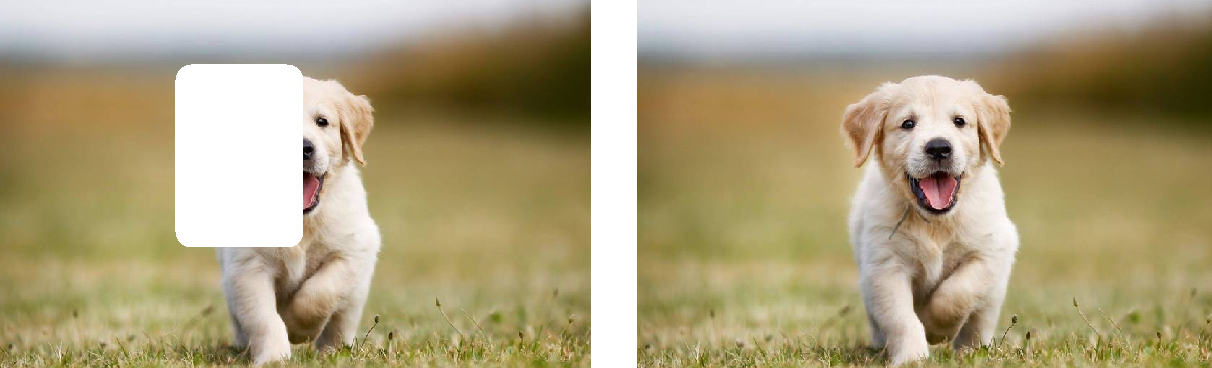
\includegraphics[width=0.6\textwidth]{imagere.png}
	\caption{Bild Rekonstruktion eines Hundes, welches durch ein Artefakt zerstört wurde}
	\label{fig:Bild40}
\end{figure}
\newpage
\subsection{Datenformat Punktwolken}\label{sec:punktwolken}

Punktwolken sind eine Menge von N Punkten, welche im Vektorraum dargestellt werden können. Jeder Punkt n $\in$ N wird durch seine (x,y,z) Koordinaten im Euklidischen Raum dargestellt. Punkten können zusätzliche Features gegeben werden, wie Farbe oder Material. Es gibt unterschiedliche Dateiformate, welche für die Abspeicherung von Punktwolken herangezogen werden können, Bespiele dafür sind PLY, STL oder OBJ. Das Polygon File Format(PLY) speichert die einzelnen Koordinaten in einer Liste, welche Vertex List genannt wird. Abb. \ref{fig:Bild7} kann eine Beispieldatei entnommen werden, in der dieser Aufbau dargestellt ist. 
\\
\begin{figure}[htbp] 
	\centering
	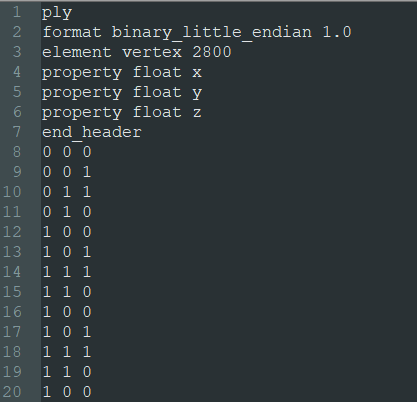
\includegraphics[width=0.4\textwidth]{plyexample.png}
	\caption{Polygon File Format}
	\label{fig:Bild7}
\end{figure}
\\
Punktwolken können als Menge betrachtet werden. Die jeweiligen Punkte sind geordnet in dieser Listen gespeichert. Jedoch spielt es keine Rolle für den Punktwolkencompiler bei der Visualisierung der Liste, auf welcher Listenposition ein jeweiliger Punkt geführt wird. Die Liste wird jedes mal gleich angezeigt, unabhängig davon, welche Permutation der einzelnen Punkte auf der Liste durchgeführt wird. Abb. \ref{fig:Bild8} kann eine visualisierte Punktwolke eines Tabakblattes entnommen werden. 
\\
\begin{figure}[htbp] 
	\centering
	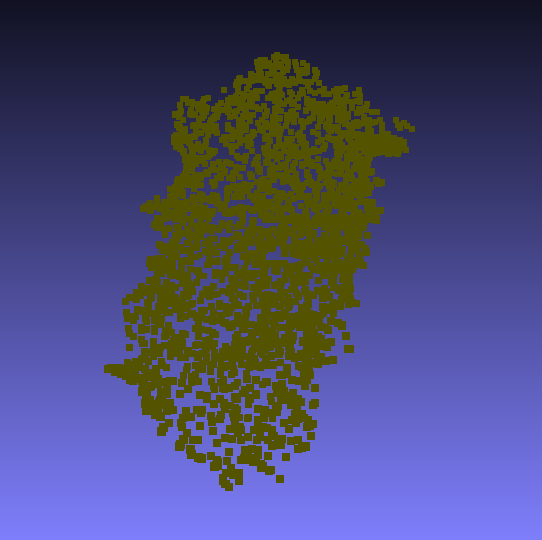
\includegraphics[width=0.5\textwidth]{leaf1.png}
	\caption{Visualisierte Punktwolke eines Tabakblattes}
	\label{fig:Bild8}
\end{figure}
\newpage
\subsubsection{Datenaufnahme von Tabakpflanzen}
~\\\\
Die Punktwolken können beispielsweise vom TERRA-REF Feld Scanner der University von Arizona Maricopa Agricultural Center and USD Arid Land Researh Station in Maricopa aufgenommen werden. Auf Abb. \ref{fig:Bild9} ist rechts eine Skizze dargestellt. Auf Abb. \ref{fig:Bild9} links ist der Scankopf des TERRA-REF dar gestellt.
\begin{figure}[htbp] 
	\centering
	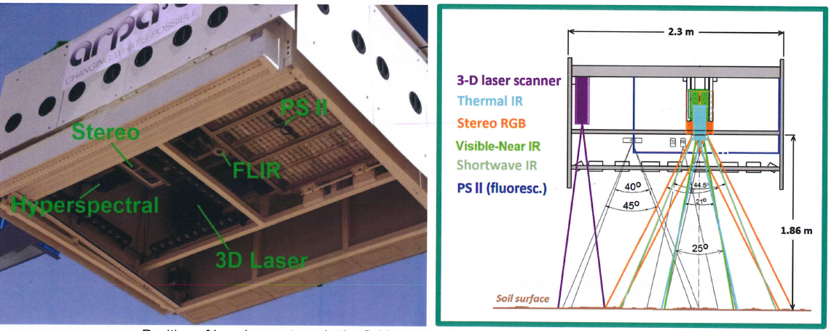
\includegraphics[width=0.5\textwidth]{lematech_2.png}
	\caption{Scankopf und Scanaufbau für die 3D-Punktwolken Gewinnung}
	\label{fig:Bild9}
\end{figure}
Der 3D Laser Scanner erzeugt 3D Punktwolken. Dabei werden die Objekte durch den Scanner erfasst und eine 3D Repräsentation, welche durch Punkte in einem dreidimensionalen Koordinaten System erfasst werden können, dargestellt. Dabei wird ein Laser über das zu scannende Objekt gefahren und durch die Reflektion des Laserstrahls auf der Oberfläche des Objektes, können die x,y,z Koordinaten des jeweiligen Punktes auf dem Objekt bestimmt werden. Ein 3D-Scan einer Tabakpflanze kann Abb.\ref{fig:Bild100} entnommen werden. Diese wurden für die hier vorliegende Arbeit vom Fraunhofer-Institut für Integrierte Schaltungen zur Verfügung gestellt. Da beim Scannen eines Objektes  die Oberfläche durch andere Objekte verdeckt sein kann, wie beispielsweise beim Scannen von Tabakpflanzen, wenn Blätter es dem Scankopf nicht ermöglichen, Objekte unterhalb eben dieser zu erreichen. Daher können Scans unvollständig sein. Dieses Problem bietet Anlass für die Zielsetzung dieser Arbeit, eine Möglichkeit zu entwickeln, diese unvollständigen Punktwolken zu vervollständigen. Weitere Ausführungen zu diesem Thema finden sich in Kapitel \ref{sec:rekdaten}. 
\begin{figure}[htbp] 
	\centering
	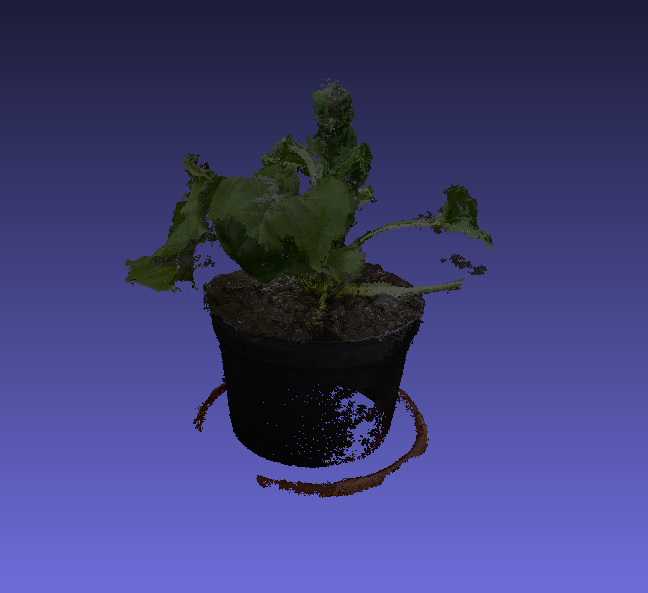
\includegraphics[width=1.0\textwidth]{plant.png}
	\caption{3D Punktwolke einer Tabakpflanze}
	\label{fig:Bild100}
\end{figure}
\newpage
\subsubsection{Die Schwierigkeit mit 3D-Data bei Machine Learning Ansätzen}\label{sec:3dprobleme}
~\\\\
Vergleicht man 3D-Data in ihrer Dimensionalität mit anderen Datenformaten, wie Bild,- Audio-, und Textdateien, ist ein erhöhter Informationsgehalt festzustellen und dadurch auch eine wesentlich höhere Komplexität in der Anwenden von Maschine Learning Algorithmen. Vor allem bei Nicht-Euklidischen 3D-Daten wie Punktwolken, welchen keine Struktur zu Grunde liegt, ist dies gegeben \cite{3dprob}.
\\\\
Wie im Kapitel \ref{sec:punktwolken} gezeigt, sind Punktwolken als Menge gespeichert, in der keine Relation untereinander besteht. Dies bedeutet, dass es für den Punktwolkencompiler nicht von Relevanz ist, auf welchem Platz die einzelnen Punkte abgespeichert werden. Die Punktwolke wird immer gleich angezeigt, egal in welcher Permutation die einzelnen Punkte abgespeichert werden. Vergleicht man nun ein Bild mit 512 Pixeln und 3 RGB-Farbkanälen, ist eine Dimension von 391680 erreicht. Vergleicht man dies mit einer Punktwolke in einem 125 cm\textsuperscript{3} großen Bereich. Da die einzelnen Koordinaten eines Punktes als rationale Zahlen dargestellt werden und diese abzählbar unendlich sind, ist auch der Suchraum unendlich groß. Dies führt zu einem erheblichen Mehraufwand für Machine Learning Ansätze, wie Deep Learning für Punktwolken.
\\\\
Im Bereich Deep Learning haben besonders die, in Kapitel Convolutional Neural Network beschrieben, Convolutional-Layer einen großen Beitrag zum Fortschritt von Deep Learning geleistet \cite{conv_adv}. Da sie helfen, die Strukturen von strukturierten Daten zu lernen und den latenten Raum zu entdecken. Da Pointclouds jedoch unstrukturiert sind, hilft es nicht unbedingt dieses Tools auch bei Punktwolken einzusetzen.
\newpage
\section{Methoden}
In diesem Kapitel werden die Methoden für die Versuchsaufbauten 1 und 2 aufgezeigt, welche mit den Fragestellungen 1 und 2 überprüft werden sollen, die unten festgehalten wurden.
\begin{description}
	\item[Fragestellung 1]
	Können durch GANs 3D-Punktwolken von Tabakblättern erlernt werden, um neue Datensätze zu generieren?\\
	
	\item[Fragestellung 2] Können durch GANs 3D-Punktwolken von Tabakblättern, die von ihrem Urzustand abgebracht wurden, rekonstruiert werden? 
\end{description}
Die Fragestellung beinhaltet, ob mit Hilfe von GANs der latente Objektraum eines Tabakblattes gelernt werden kann und anschließend durch den Generator des GAN, Tabakblätter erzeugt werden können. Dieser Versuchsaufbau wird in Kapitel \ref{sec:versuch1-aufbau} behandelt. Die dazugehörigen Trainingsdaten werden in Kapitel \ref{sec:versuch1-traingsdaten} vorgestellt. Bei Fragestellung 2 soll überprüft werden, ob es mit Hilfe von GAN möglich ist, Artefakte von Tabakblätter zu entfernen und den Urzustand wieder herzustellen.  Dieses Verfahren wurde in Kapitel \ref{sec:rekdaten} beschrieben. Die Trainingsdaten für diesen Versuchsaufbau können Kapitel \ref{sec:versuch2_daten} entnommen werden. 
\\\\
Versuchsaufbau 1.2 und 2.1 wurden auf einem Computer mit Ubuntu 14.05 Betriebssystem, mit einem IntelR CoreTM i7-7700k mit 4.50GHz und einer Geforce GTX 1080 mit 8G Grafikspeicher durchgeführt. Training und Test  wurden mit CUDA 9.0 und cudNN 7.1.1 durchgeführt. Als Programmiersprache wurde Python 2.7, beziehungsweise 3.5 für Datengenerierung, verwendet. Als ANN Libary wurde Tensorflow 1.5 genutzt und TFlearn 0.3.2. Für die EMD und Chamfer Loss des Autoencoder wurde die Implementierung von dfanhqme (https://github.com/fanhqme/PointSetGeneration) benutzt.
\\\\
Versuchsaufbau 1.1 und 2.2  wurden auf einen Computer mit Windows Betriebssystem, mit einem IntelR CoreTM i7-7700k mit 4.50GHz und einer Geforce GTX 1080 mit 8G Grafikspeicher durchgeführt. Training und Test wurden mit CUDA 9.0 und cudNN 7.1.1 durchgeführt. Als Programmiersprache wurde Python 3.5 verwendet. Als ANN Libary wurde Tensorflow 1.10 genutzt.
\newpage

\subsection{Datensatz 1. Versuchsaufbau}\label{sec:versuch1-traingsdaten}

Der erste Datensatz ``Stühle`` besteht aus 6778 Punktwolken, mit jeweils 2048 Punkten. Dieser wurde dem Shapenet Datensatz (www.shapenet.org) entnommen. Die Daten sind im PLY Datenformat abgespeichert. Ein Beispielpunktwolke kann aus Abb. \ref{fig:Bild50} entnommen werden. Der Datensatz wurde auch in der Arbeit von Achlioptas, Diamanti, Mitliagkas und Guibas \cite{3dgan} verwendet, was in Kapitel \ref{sec:3dgan} bereits vorgestellt wurde. In der hier vorliegenden Arbeit dient er als Validierungsdatensatz, um die Qualität der generierten Daten des GAN, welches mit Tabakblättern trainiert wurde, zu vergleichen.
\\\\
Die Daten für den zweiten Datensatz ``Blätter`` stammen vom Fraunhofer-Institut und deren Gewinnung wurde in Kapitel \ref{sec:punktwolken} beschrieben. Der Grunddatensatz bestand aus mehreren 3D-Scans von Tabakpflanzen, bei welchen die Blätter der Pflanze zu einem Datensatz zusammengefügt wurden. Der ``Blätter`` Datensatz besteht aus 422 Punktwolken, welche dann durch ein Punktreduktionsverfahren auf jeweils 2048 Punkten je Punktwolke reduziert worden sind. Aus Komplexitätsgründen wurden der Farbchannel in dieser Arbeit außen vor gelassen, um den Informationsgehalt der Daten zu reduzieren und ein Training zu vereinfachen. Außerdem spielen Farben beim derzeitigen Ziel der Arbeit, Rekonstruktion von Tabakblättern, keine Rolle und nehmen keinen Einfluss auf die Verwendbarkeit des Ergebnisses. Abgespeichert wurden die Daten im PLY-Datenformat.

\begin{figure}[htbp] 
	\centering
	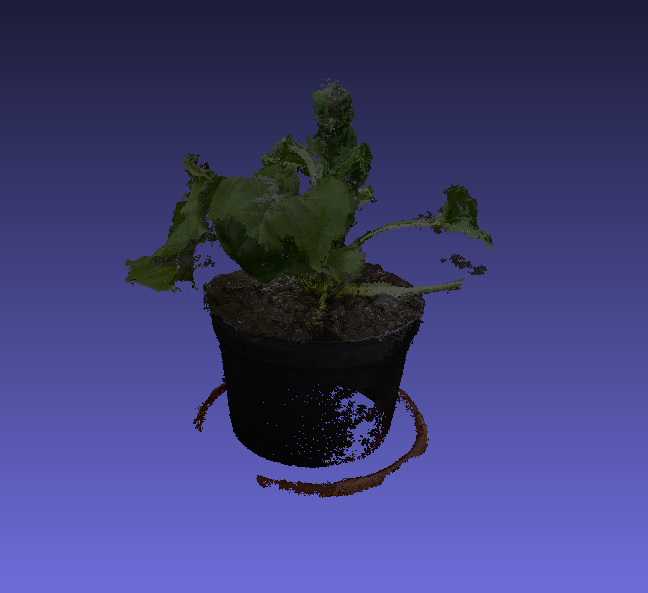
\includegraphics[width=0.6\textwidth]{plant.png}
	\caption{3D Punktwolke einer Tabakpflanze}
	\label{fig:Bild50}
\end{figure}

\begin{figure}[htbp] 
	\centering
	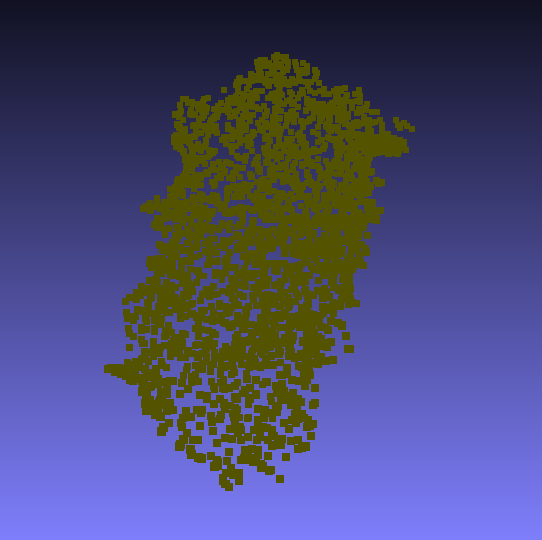
\includegraphics[width=0.5\textwidth]{leaf1.png}
	\caption{3D Punktwolke eines Tabakblattes mit 2048 Punkten}
	\label{fig:Bild51}
\end{figure}
\newpage
\subsection{Datensatz 2. Versuchsaufbau}\label{sec:versuch2_daten}

Für den zweiten Versuchsaufbau wurde auf den Datensatz aus Versuchsaufbau 1. Datensatz ``Blätter`` zurück gegriffen. Der Grunddatensatz besteht aus 422 unterschiedlichen Blättern. Dieser Datensatz wird nun dahingehen verändert, dass Löcher in die Blattoberfläche eingefügt werden. Diese Löcher simulieren das beim Scanverfahren die Sicht des Scanners auf das Blatt durch andere Blätter verdeckt war und diese somit unvollständig eingescannt wurden. Dieses Verdecken wir durch 3D-Sphären simuliert, wie in Abb. \ref{fig:Bild52}  rot dargestellt. Die Sphären bestehen aus 10 000 Punkten, welche alle einen maximalen Radius von 15 mm haben und alle aus einer Normalverteilung entnommen werden, um  eine gleichmäßige Verteilung der Punkte zu gewährleisten. Die Sphären werden nun vom Koordinatenursprung im euklidischen Raum bewegt, so dass sich 46 unterschiedliche Sphären im Raum ergeben. Diese werden dahingehend im Raum bewegt, um möglichst eine hohe Differenzmenge zu den 422 Blättern im Datensatz zu haben. In Abb. \ref{fig:Bild53} sind alle Sphären symbolisch eingefügt, um dieses Vorgehen zu veranschaulichen. Um das Verdecken zu simulieren, wird die Differenzmenge je Blatt mit einer der Sphären errechnet. Wobei sich in der Differenzmenge eines Punktes der nächste Nachbar in einem Radius von 3 mm befindet. Durch dieses Verfahren entstehen kreisförmige Löcher in den Blättern, was auf Abb. \ref{fig:Bild54} dargestellt ist. Anschließend werden alle erzeugten ``zerstörten`` Blätter nach der Anzahl ihrer übrig geblieben Punkte gefiltert, um zu gewährleisten, dass genügen Punkte aus dem Urblatt entfernt worden sind und eine visuelle Diskrepanz zwischen den Blätter vorhanden ist. Dieses Vorgehen hat letztendlich zu 2047 zerstörten Blättern, mit jeweils 2048 Punkten geführt.

\begin{figure}[htbp] 
	\centering
	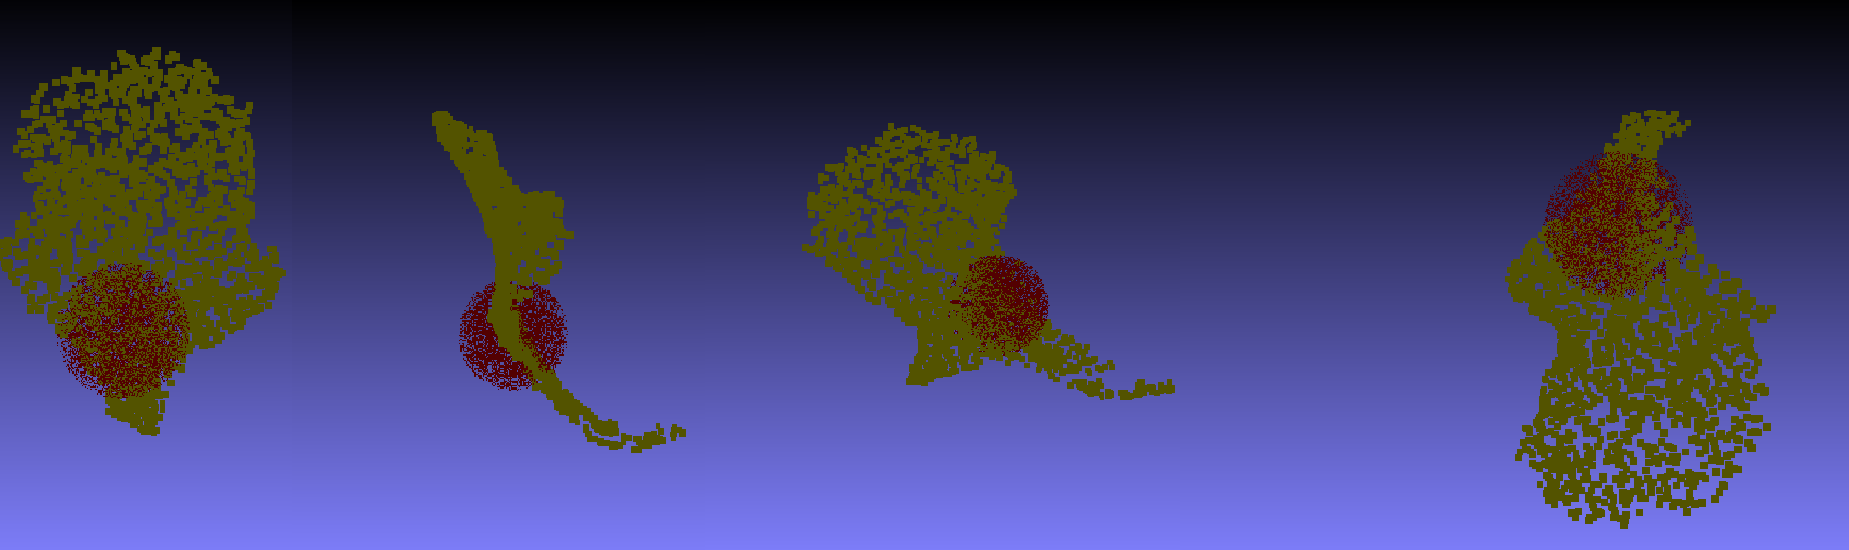
\includegraphics[width=1.0\textwidth]{sphere1.png}
	\caption{Tabakblatt mit Sphäre, welche die Differenzmenge bilden}
	\label{fig:Bild52}
\end{figure}

\begin{figure}[htbp] 
	\centering
	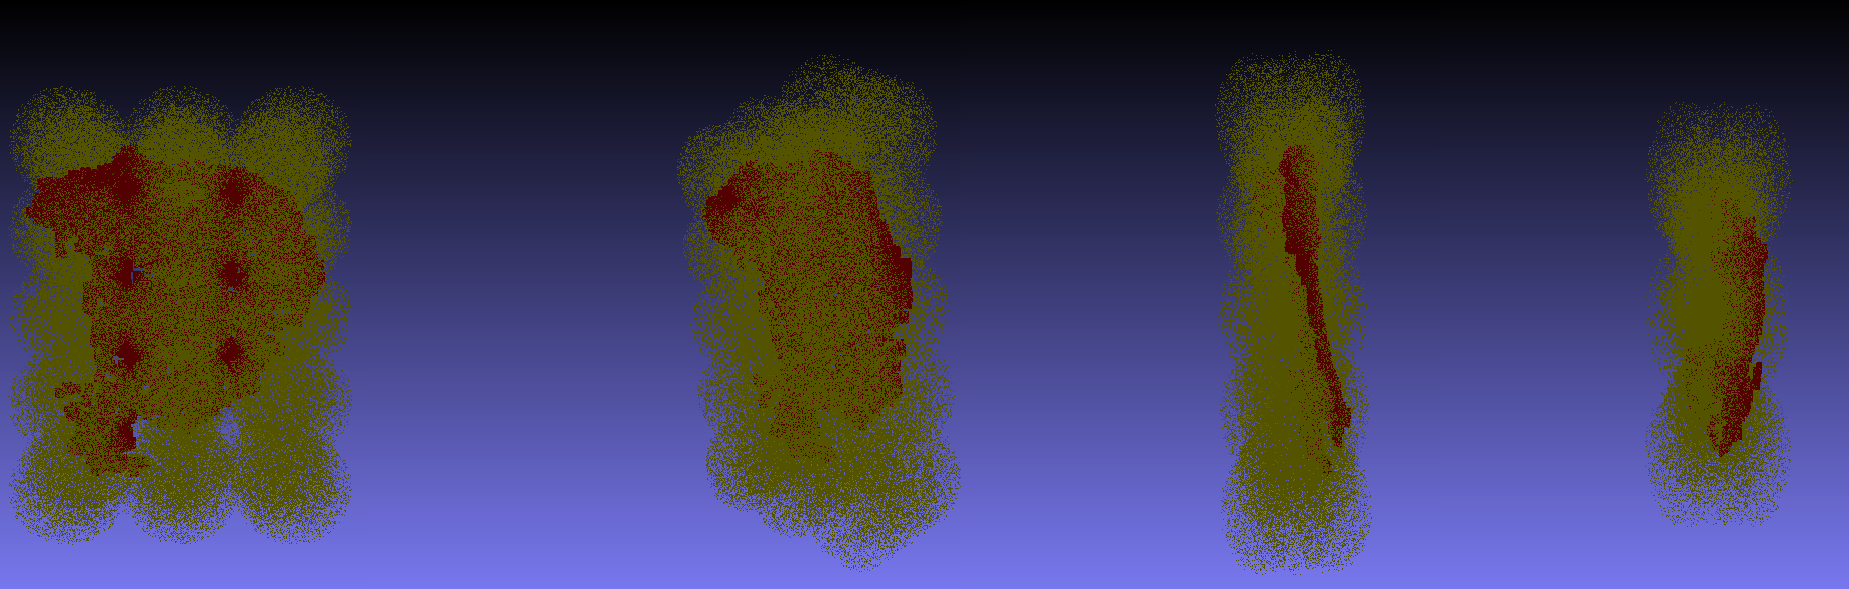
\includegraphics[width=1.0\textwidth]{allsphere.png}
	\caption{Sphäre im Raum, welche das Verdecken der Blätter simuliert}
	\label{fig:Bild53}
\end{figure}

\begin{figure}[htbp] 
	\centering
	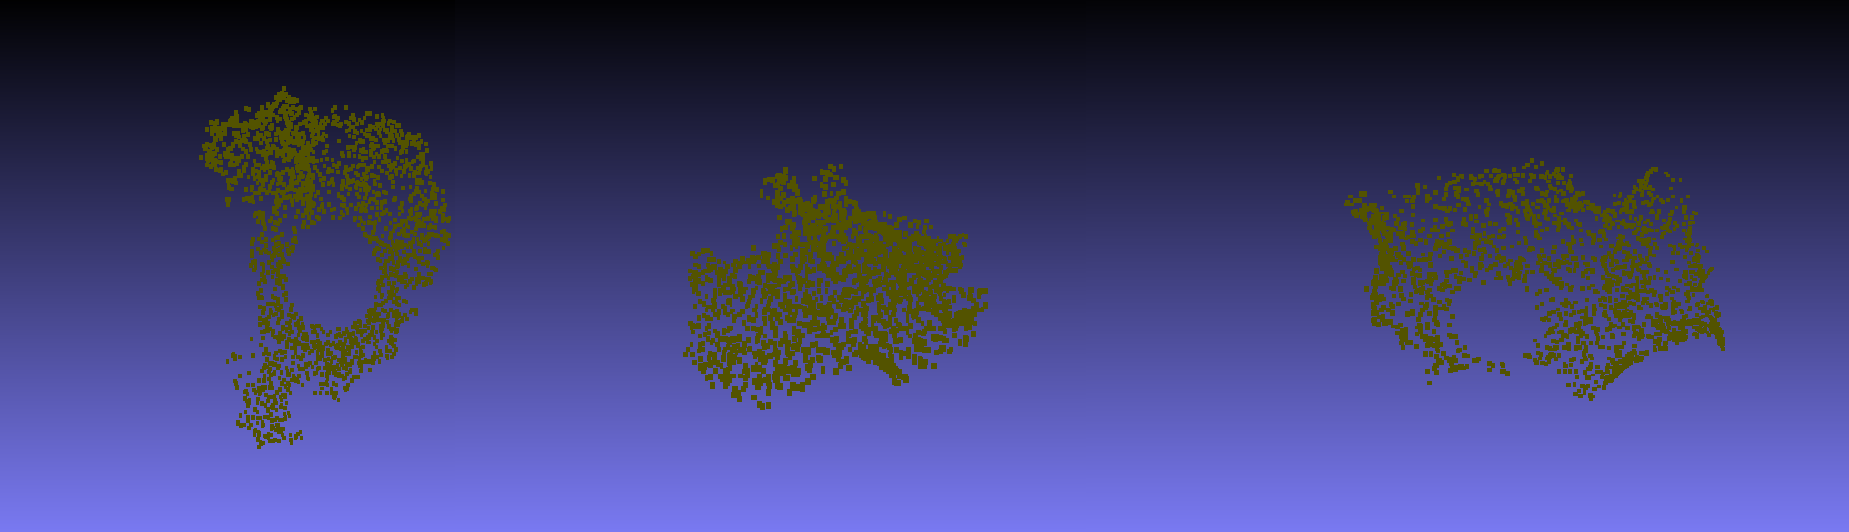
\includegraphics[width=1.0\textwidth]{training_destroyed.png}
	\caption{3D Punktwolke von zerstörten Tabakblättern}
	\label{fig:Bild54}
\end{figure}
\newpage


\subsection{Versuchsaufbau 1 - GAN}\label{sec:versuch1-aufbau}

Der Versuchsaufbau 1 besteht aus zwei unterschiedlichen Versuchen. Aufbau 1.1 ist das RAW-GAN \cite{3dgan}), dabei wird auf den Vanilla-GAN Aufbau zurückgegriffen. Die Meta Trainingsvariablen für diesen Versuch sind eine Learningrate mit 0,0005 und einem Adam Optimizer, welcher zu den Mini-Batch Gradient Descent Verfahren aus Kapitel \ref{sec:test} gehört und dabei auf das aus Kapitel \ref{sec:momentum}, zurückgreift, mit einem Beta1 von 0,5 und einem Beta2 von 0,5. Die Batchgröße ist 64. Der Discriminator besteht aus 5-Layern, welche aus 1-Dimensionalen Convolutional-Layern bestehen, mit einer Filteranzahl [64, 128, 256, 256, 512] je Layer. Mit einer Kernel Größe von 1 und Stride von 1. Als Aktivierungsfunktion wird die ReLu-Funktion genutzt. Darauf folgen 3 Fully-Connected-Layer, mit der Größe [128, 64, 1], alle mit einer ReLu-Funktion. Der Generator des RAW-GAN besteht auf 6 Fully-Connected-Layern, mit [64, 128, 512, 1024 ,1536 ,6144] Neuronen, jeweils mit der ReLu Aktivierungsfunktion. Der Noisevektor z wird aus einer 128-D Normal Verteilung entnommen, mit $\mu$ = 0 und $\sigma$ =  0,2. Als Zielfunktion wird die Wasserstein Metric gewählt, da diese bessere Ergebnisse im Versuchsaufbau von Achlioptas, Panos und Diamanti \cite{3dgan} erzielt hat. Das Training erfolgt jeweils mit den Datensätze ``Stühle`` und ``Blätter``, wie in Kapitel \ref{sec:versuch1-traingsdaten} beschrieben.
\\\\
Der Versuchsaufbau 1.2 ist das Latent-GAN, welches in Kapitel \ref{sec:3dgan} bereits vorgestellt wurde. Es wurde die Implementierung von \cite{3dgan} verwendet $(www.github.com/optas/latent_3d_points)$. Zunächst wird dabei der Autoencoder mit den Trainingsdaten trainiert. Das Training erfolgt mit einer Learningrate von 0,0005 und einer Nachsitze von 50. Der Encoder besteht dabei aus 4 1-D Convolutional-Layern mit [64, 128, 246, 1024] Filtern, einem Stride von 1 und Size von 1. Die Batchgröße ist 64. Als Aktivierungsfunktion wir die ReLu verwendet. Der Encoder besteht aus 3 Fully-Connected-Layern mit [256, 256, 6144] Neuronen, alle mit der ReLu-Zielfunktion. Das Training erfolgt jeweils mit den Datensätze ``Stühle`` und ``Blätter``, wie in Kapitel \ref{sec:versuch1-traingsdaten} beschrieben und wurde auf 500 Epochen durchgeführt. Nach dem Training des Autoencoder kann der komprimierte Latent Code, welcher von Encoder erstellt wird, dazu verwendet werden, das Latent-GAN zu trainieren. Alle Trainingsdaten werden nun durch den Encoder komprimiert, um ihren 128-D Latenten Code y zu erzeugen. Mit diesem wird nun das GAN trainiert, um eigene Latente Codes zu produzieren, welche vom Decoder wieder auf ihre ursprüngliche Dimension von 2048 Punkten projiziert werden. In Abb. \ref{fig:Bild39} ist dieser Prozess dargestellt. Der Generator des Latent-GAN besteht aus 2 Fully-Connected-Layern mit [128, 128] Neuronen, welche als Aktivierungsfunktion eine ReLu-Funktion benutzen. Der Noisevektor z wird aus einer 128-D Normal Verteilung entnommen, mit $\mu$ = 0 und $\sigma$ =  0,2. Der Discriminator besteht aus [128, 64, 1] Fully-Connected-Layern, welche ebenfalls ReLu-Funktion nutzen. Als Zielfunktion wird die Wasserstein Metrik gewählt, da diese bessere Ergebnisse im Versuchsaufbau von Achlioptas, Panos und Diamanti\cite{3dgan} erzielt hat. 

\subsection{Versuchsaufbau 2 - CGAN für Punktwolkenrekonstruktion }\label{sec:versuch2-aufbau}

Da im Versuchsaufbau 1 das Latent-CGAN bessere Ergebnisse beim Erlernen von Punktwolken-Daten liefert, wird im Versuchsaufbau 2.1 Latent-CGAN das Komprimieren von Trainingsdaten übernommen und dahingehend verändert, das Ziel von C-GAN zu übernehmen und bedingte Wahrscheinlichkeiten zu erlernen. Zunächst werden, wie auch bei Versuchsaufbau 1, die Trainingsdaten vgl. \ref{sec:versuch2_daten} an einem Autoencoder trainiert. Dabei wird jeweils ein Autoencoder für zerstörte Blätter heran genommen und einer für unzerstörte im Urzustand.
\\\\
Die Autoencoder folgen dabei dem gleichen Aufbau wie in Versuchsaufbau 1.2. Der Encoder besteht dabei aus 4 1-D Convolutional-Layern mit [64, 128, 246, 1024] Filtern, einem Stride von 1 und Size von 1. Als Aktivierungsfunktion wird die ReLu-Funktion verwendet. Der Decoder besteht aus 3 Fully-Connected-Layern mit [256, 256, 6144] Neuronen, alle mit der ReLu-Zielfunktion. Als Batchsize wird 64 genommen. Als Zielfunktion wird jeweils einmal die CD getestet und die EMD. Für den Autoencoder wurde die Implementierung von \cite{3dgan} verwendet$(www.github.com/optas/latent_3d_points)$. 
\\\\
Der Generator des Latent-CGAN bekommt als Input z einen 128-D Vektor, welcher aus einer Normal Verteilung mit $\mu$ = 0 und $\sigma$ =  0,2 entnommen wurde. Y, welches zusätzlich zu z dem Generator zum Training eingespeist wird, sind die vom Autoencoder codierten 128-D komprimierten, zerstörten Tabakblätter. Der Generator des Latent-GAN besteht aus 2-Fully-Connected-Layer mit [128, 128] Neuronen, welche als Aktivierungsfunktion eine Leaky-ReLu-Funktion benutzen. Der Discriminator besteht aus 2 Fully-Connected-Layern mit der Größe [128, 128]. Der Discriminator bekommt als Input entweder den vom Generator erzeugten latenten Code x', welcher vom Encoder des Autoencoder zu einem unzerstörten Blatt gemappt werden kann und zusätzlich y, also (x',y). Oder ein aus den Trainingsdaten stammendes (x,y) Paar, welche als reale-Datensätze gekennzeichnet ist. Als Ziel wird jeweils die Wasserstein Metrik und die Vanilla-GAN Metrik Loss-Function benutzt. Beim Trainingsaufbau 2.2 RAW-CGAN bekommt der Generator als Input Noisevektor z einen 128-D Vektor, aus einer  Normal Verteilung, entnommen mit $\mu$ =  0 und $\sigma$ =  0,2. Des Weiteren wird als y dem Generator die zerstörte Blatt Punktwolke, welche als ein 6144-D Vektor dargestellt ist, als Input übergeben. Der Generator besteht aus Fully-Connected-Layern mit [6272, 3163, 1568, 3136, 4850, 5680, 6144] Neuronen je Layer. Als Aktivierungsfunktion wird die Leaky-ReLu genommen. Im letzten Layer wird keine Aktivierungsfunktion verwendet, um den Output linear verarbeitbar zu machen und damit Euklidische Koordinaten generiert werden können. Des Weiteren wird nach jedem Layer ein Batch-Normalisation-Layer eingesetzt, mit Momentum 0,9 und einem Beta1 und Beta2 von 0,5. Der Discriminator besteht aus [12288, 6144, 3072,1536, 768, 384, 128, 32, 1] Fully-Connected-Layern mit Aktivierungsfunktion Leaky-ReLu. Bis auf den letzten Layer, in welchem die Sigmoid-Funktion verwendet wird, wenn als Zielfunktion die Vanilla-GAN gewählt wird. Bei Verwendung der Wasserstein Metrik wird auf eine Aktivierungsfunktion verzichtet. Des weiteren wird nach jedem Layer ein Batch-Normalisation-Layer eingesetzt, mit Momentum 0.9 und einem Beta1 und Beta2 von 0,5. Der Input des Discriminators ist die vom Generator erstellte (x',y), oder die direkt aus den Trainingsdaten stammenden Punktwolken Paare des zerstörten Blatts y und Urzustand Blatts x als Tupel (x,y).Als Zielfunktion wird die Vanilla-GAN und W-GAN Zielfunktion getestet.
\\\\
Im weiteren Versuchsaufbau für den RAW-CGAN wird der Discriminator umgebaut, um ihm durch Convolutional-Layer bessere Lernfähigkeiten zu geben. Dies sorgt nicht nur für Vorteile für den Discriminator, sondern dadurch kann auch der Generator durch den Gradienten des Discriminators einen besseren latenten Raum lernen. Der Generator bleibt in diesem Aufbau gleich, der Discriminator bekommt [64, 128, 256, 256, 512] 1-D-Convolutional-Layer, mit einer Kernel-Größe von 1 und Stride von 1. Als Aktivierungsfunktion wird eine Leaky-ReLu verwendet und die Batchsize beträgt 64. Anschließend folgen [128, 32, 1] Fully-Connected-Layer mit Leaky-ReLu. Zwischen jedem Layer befindet sich ein Batch-Normalisation-Layer mit Momentum von 0,9 und einem Beta1 und Beta2 von 0,5. Abb. \ref{fig:Bild55} kann der Aufbau und die Konnektivät der einzelnen Komponenten entnommen werden.

\begin{figure}[htbp] 
	\centering
	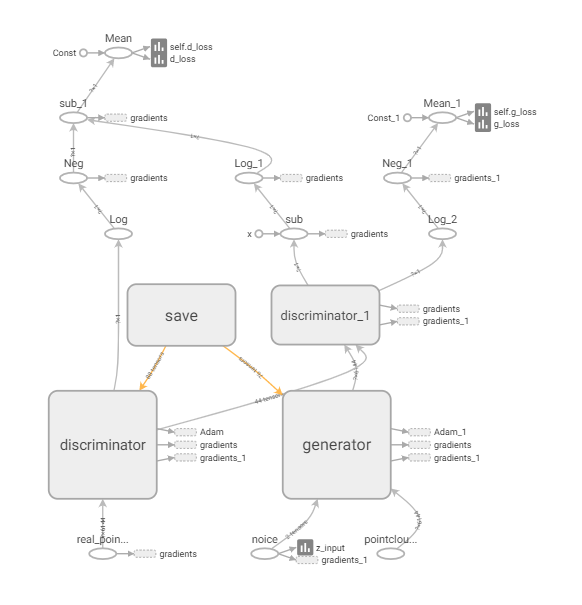
\includegraphics[width=0.7\textwidth]{point-cgan.png}
	\caption{Aufbau des RAW-CGAN}
	\label{fig:Bild55}
\end{figure}
\newpage

\section{Evaluation und Ergebnisse}

In diesem Kapitel wird auf die Ergebnisse von Versuchsaufbau 1 und 2 eingegangen. Zunächst wird Versuchsaufbau 1, vgl. \ref{sec:versuch1-aufbau} das Erlernen von latentem Raum von Punktwolken, vorgestellt. Dabei wird ein Vergleich zwischen dem Modeldatensatz ``Stühle``, sowie einem aus der Praxis stammenden Datensatz ``Blätter``, aufgezeigt. Anschließend wird auf die Ergebnisse aus Versuchsaufbau 2, vgl. \ref{sec:versuch2-aufbau}, eingegangen. Dabei wird evaluiert, ob es möglich ist, den Urzustand der zerstörten Blattdaten wieder herzustellen und ob aussagekräftige Ergebnisse für die Anwendbarkeit in der Praxis gewonnen werden können. Da es keine gängigen Validierungsmethoden, beziehungsweise Validierungsmetriken gibt, wird sich bei der Prüfung der Testergebnisse auf das menschliche Auge verlassen, so dass die Prüfung in Form einer Sichtprüfung erfolgt.

\subsection{Ergebnisse - Versuchsaufbau 1}

Von RAW-GAN, aus dem Versuchsaufbau 1.1 auf Basis der Blattdaten, lassen sich nach 500 Trainingsepochen die auf  Abb.\ref{fig:Bild100} aufgezeigten Beispieldatensätze erkennen, welche vom Generator erzeugten wurden. Wie festzustellen ist, reicht die Qualität der Blätter nicht für eine Weiterverarbeitung aus. Der latente Raum, welcher von den GAN erlernt wurde und am Ende durch den Generator produziert wurde, zeigt keine Ähnlichkeit zu normalen Blättern, welche im Datensatz enthalten waren. Die Daten erinnern eher an einen hohlen Ball, denn an Blättern. Es formen sich Punktansammlungen in der Nähe des Koordinatenursprungs und es lassen sich kein Anzeichen für das Bilden einer Blattfläche erkennen.
\begin{figure}[htbp] 
	\centering
	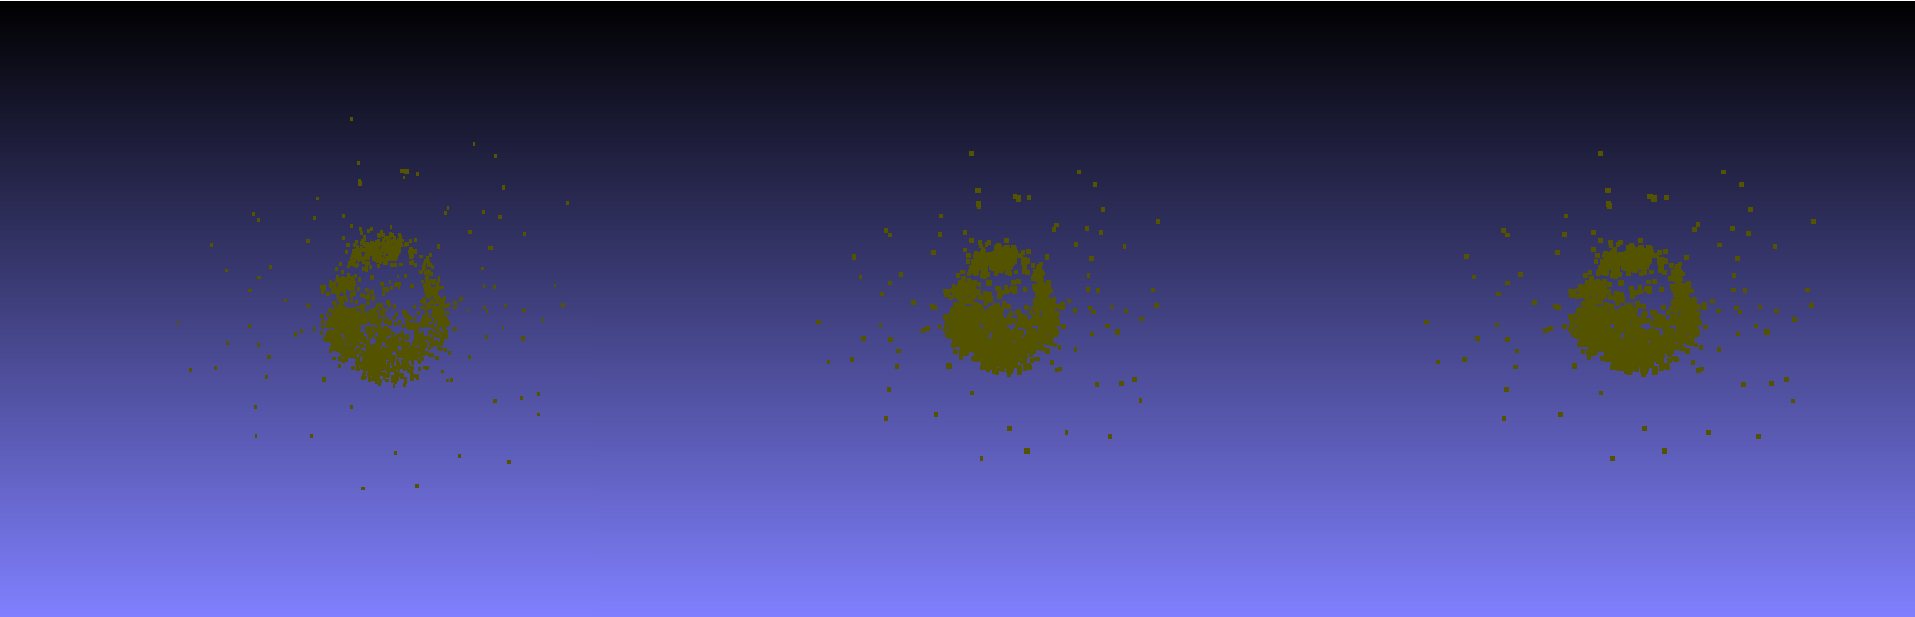
\includegraphics[width=1.0\textwidth]{raw_gan_leaf_example.png}
	\caption{Generierte Beispieldaten vom Generator des RAW-GAN mit den Blattdaten}
	\label{fig:Bild100}
\end{figure}
Die starken Punkthäufungen am Koordinatenursprung ergeben sich dadurch, dass die realen Blattdaten an dieser Stelle häufig vertreten sind, sich an den Blattkanten jedoch eher unterscheiden. So lernt der Generator, an diesen vermehrt auftretenden Schnittpunkten auch mehr Punkte zu generieren, als außerhalb. Dieser Effekt ist auf Abb. \ref{fig:Bild81} zu erkennen. Dargestellt sind 24 Datensätze aus dem Blattdatensatz, welche aus verschiedenen Blickwinkeln in ein Koordinatensystem geladen wurden. Die Punkte häufen sich in der Nähe des Koordinatenursprungs und sind im äußeren Bereich weniger frequentiert verteilt.  
\begin{figure}[htbp] 
	\centering
	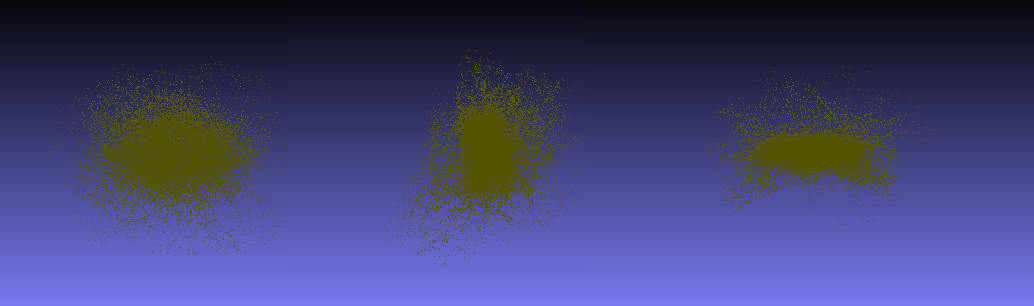
\includegraphics[width=1.0\textwidth]{ansammlung.png}
	\caption{24 Punktwolken aus dem Blattdatensatz in einen Koordinatensystem}
	\label{fig:Bild81}
\end{figure}
Vergleicht man dies mit Abb.\ref{fig:Bild100}, sind dort ebenfalls dichte Ansammlungen zu erkennen. Der W-GAN Loss für den Generator und Discriminator kann Abb. \ref{fig:Bild1002} entnommen werden. Dass der Loss des Discriminators konstant über mehrere Epochen bleibt, lässt sich daraus schließen, dass der Critic keine Schwierigkeiten damit hat, die beiden Datenverteilungen zu unterscheiden. Es ist kein Anzeichen von Verbesserung zu Erkennen wenn das Training länger als 500 Epochen läuft. 
\begin{figure}[htbp]
	\centering
	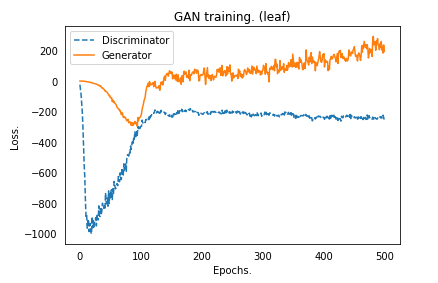
\includegraphics[width=0.5\textwidth]{raw_gan_leaf_result.png}
	\caption{Trainingsverlauf des RAW-GAN mit den Blattdaten}
	\label{fig:Bild1002}
\end{figure}
~\\\\
Ähnliche Ergebnisse sind auch beim RAW-GAN von Versuchsaufbau 1.1 mit den Stuhldaten zu beobachten. Wobei die Qualität der Stühle stärker an die im Trainingsdatensatz enthalten Daten erinnert, vgl. Abb. \ref{fig:Bild58}. Es zeichnen sich Lehne und Stuhlbeine in den Daten ab, die vom GAN trainierten Generator stammen. Der Trainingsverlauf ist Abb. \ref{fig:Bild57} zu entnehmen. Dabei ist zu sehen, dass der Discriminator sich nicht mehr verbessert und der Generator keine besseren Ergebnisse liefern kann. Diese Ergebnisse decken sich mit den von Achlioptas, Panos und Diamanti \cite{3dgan} festgestellten Prämissen, nach welchen das RAW-GAN keine qualitativ hochwertigen Stuhldaten erzeugen konnte.  
\begin{figure}[htbp] 
	\centering
	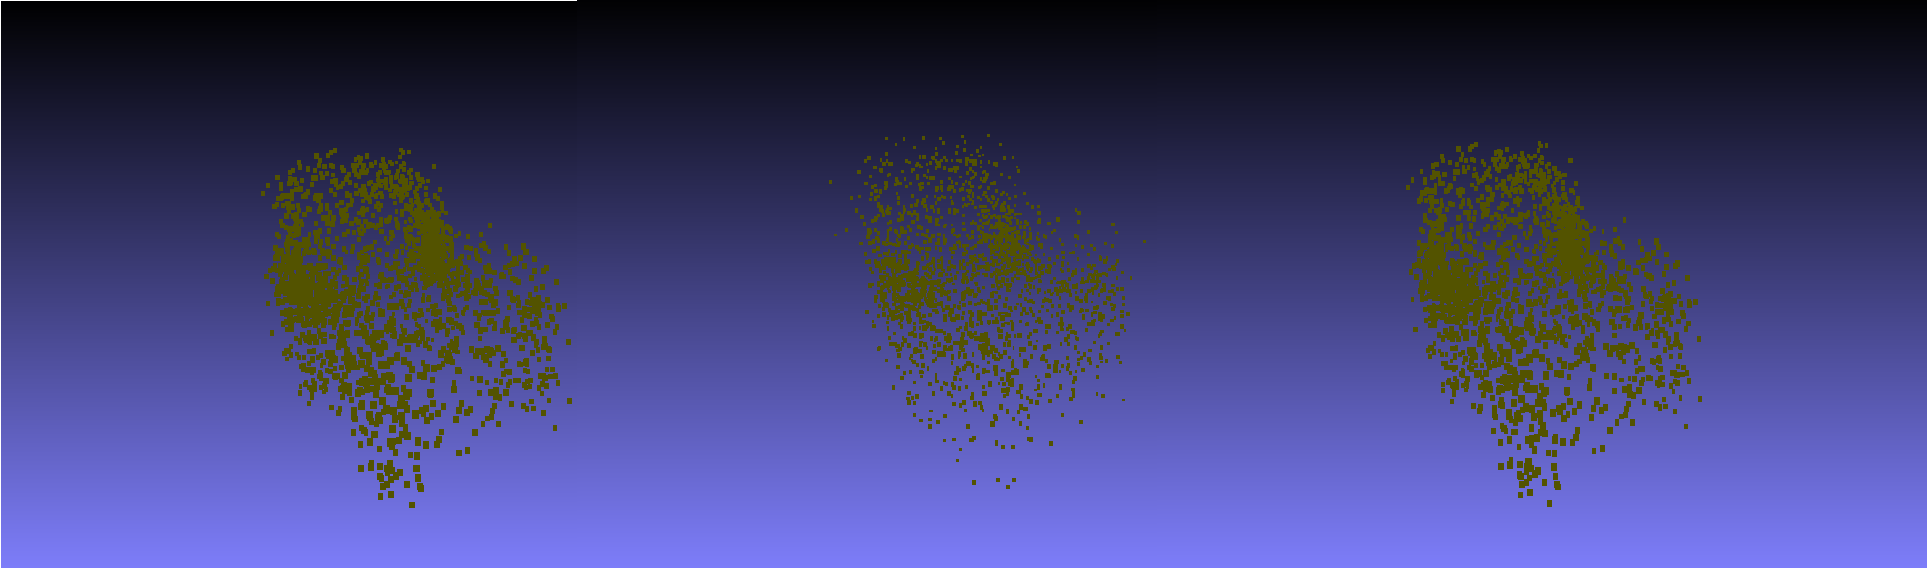
\includegraphics[width=1.0\textwidth]{raw_gan_chair_example.png}
	\caption{Generierte Beispieldaten vom Generator des RAW-GAN mit den Stuhldaten}
	\label{fig:Bild58}
	\end{figure}
\begin{figure}[htbp] 
	\centering
	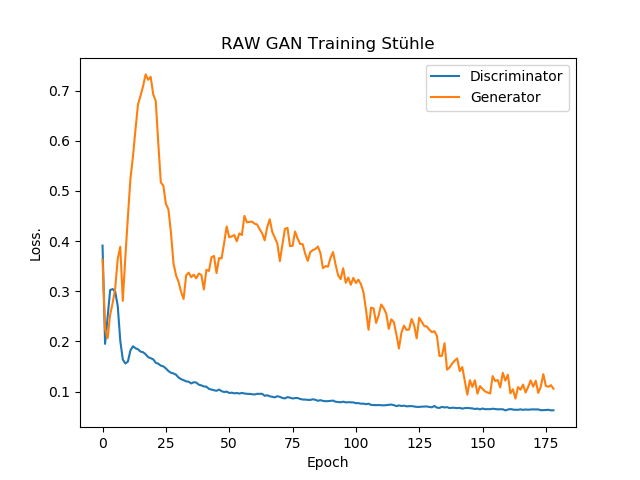
\includegraphics[width=0.5\textwidth]{raw_gan_chair_result.png}
	\caption{Trainingsverlauf des RAW-GAN mit den Stuhldaten}
	\label{fig:Bild57}
\end{figure}
\pagebreak\linebreak 
Um nun genauer zu beleuchten, was die Ursachen für den Qualitätsunterschied zwischen den beiden generierten Datensätzen ausmacht, und um festzustellen ob durch mehr Blattdaten bessere Ergebnisse erzeugt werden können, wurden die Stuhldaten auf 422 Trainingsdaten reduziert und ein erneutes Training des RAW-GAN durchgeführt. Die erzeugten Beispieldaten können Abb. \ref{fig:Bild60} entnommen werden. Vergleicht man die Qualität des RAW-GAN mit dem Training an 422 Stuhldaten und 
6778 Stuhldaten (vgl. Abb. \ref{fig:Bild58}) ist in Abb. \ref{fig:Bild60}, ist eine Steigerung der Qualität klar festzustellen. 
\begin{figure}[htbp] 
	\centering
	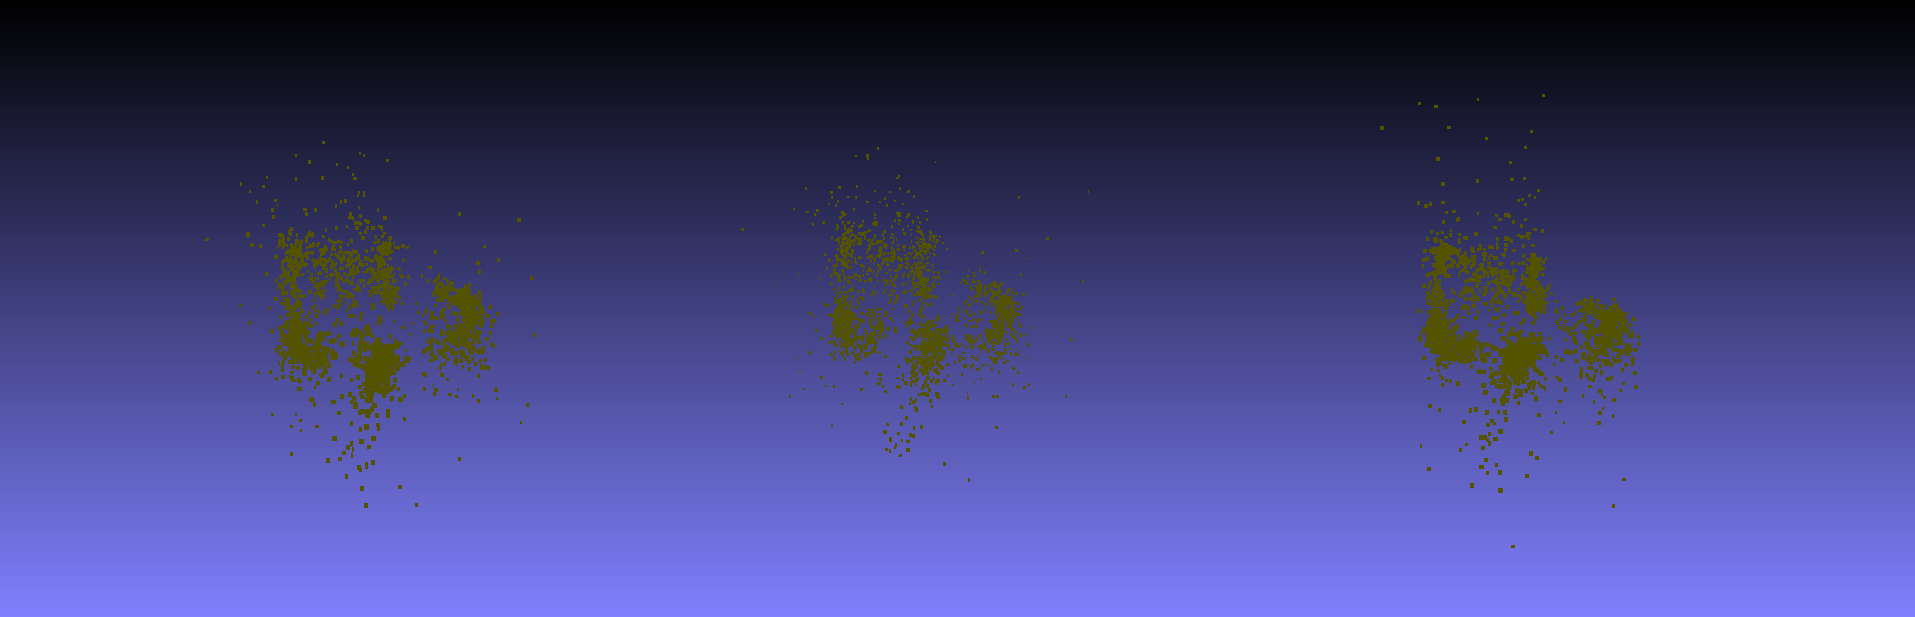
\includegraphics[width=1.0\textwidth]{raw_gan_result_400_result.png}
	\caption{Trainingsbeispiele des RAW-GAN mit den 422 Stuhldaten}
	\label{fig:Bild60}
\end{figure}
~\\\\
Für den Versuchsaufbau 1.2 Latent-GAN mit Stühlen kann der Trainingsverlauf der Abb. \ref{fig:Bild61} entnommen werden. Der Generator Loss verbessert sich zwar über mehrere Epochen gering, der Discriminator bleibt jedoch konstant auf seinem Ergebnisse und lässt keine starken Verbesserung des Generators mehr zu, da er die beiden Datenverteilungen perfekt unterscheiden kann. Dies führt dazu, dass der Generator kein Feedback über die Qualität seiner generierten Daten erhält und sich nicht verbessern kann.  
\begin{figure}[htbp] 
	\centering
	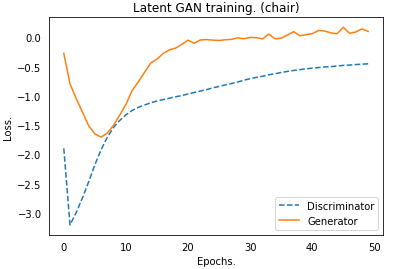
\includegraphics[width=0.5\textwidth]{latent_gan_chair_result.png}
	\caption{Trainingsverlauf des Latent-GAN mit den Stuhldaten}
	\label{fig:Bild61}
\end{figure}
Beispieldatensätze, welche vom Generator nach Beendigung des Trainings erzeugt wurden, indem der latente Code vom Generator in den Decoder als Input gegeben wurde, sind Abb. \ref{fig:Bild62} zu entnehmen. Es handelt sich dabei um qualitativ hochwertige Daten, welche eine Ähnlichkeit mit denen aus dem Trainingsdatensatz aufweisen. Die Ergebnisse decken sich mit denen von Achlioptas \cite{3dgan}, nach welchen das Latent-GAN qualitativ gute Stuhldaten erzeugen konnte.  
\begin{figure}[htbp] 
	\centering
	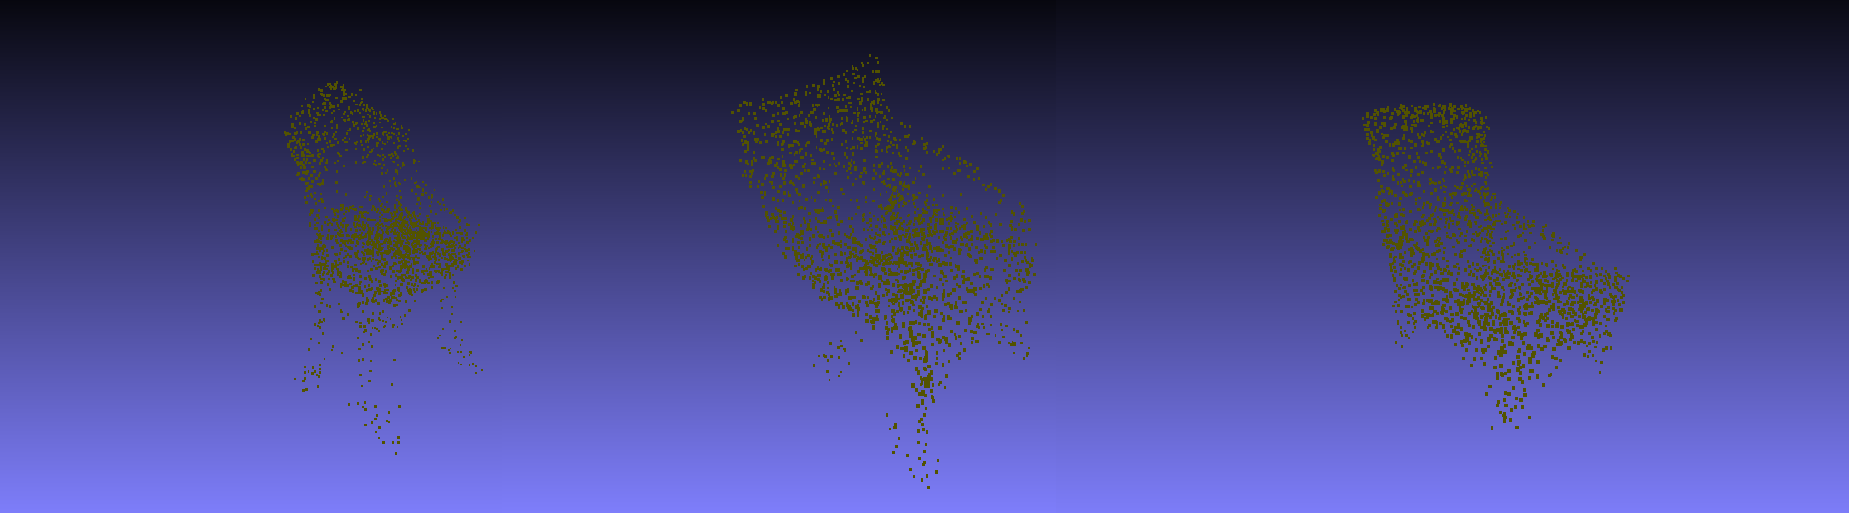
\includegraphics[width=1.0\textwidth]{latent_gan_chair_example.png}
	\caption{Trainingsbeispiele des Latent-GAN mit den Stuhldaten}
	\label{fig:Bild62}
\end{figure}
~\\\\
Für das Latent-GAN, welches mit den Blattdaten trainiert wurde, können exemplarisch generierte Daten aus der Abb. \ref{fig:Bild64} entnommen werden. Diese zeigen eine qualitative Grundfläche, welche in der Trainingsdatengesamtheit enthalten ist. Jedoch ist festzustellen, dass es starke Punkthäufungen an gewissen Bereichen je Blatt gibt. Beispielsweise zu sehen beim zweiten Blatt von rechts, auf Abb. \ref{fig:Bild64} , dort mit einem roten Kreis markiert. Der Trainingsverlauf in Abb. \ref{fig:Bild63} zeigt, dass keine starken Veränderungen im weiteren Verlauf zu erwarten sind und das Training bereits über mehrere Epochen stagniert.
\begin{figure}[htbp] 
	\centering
	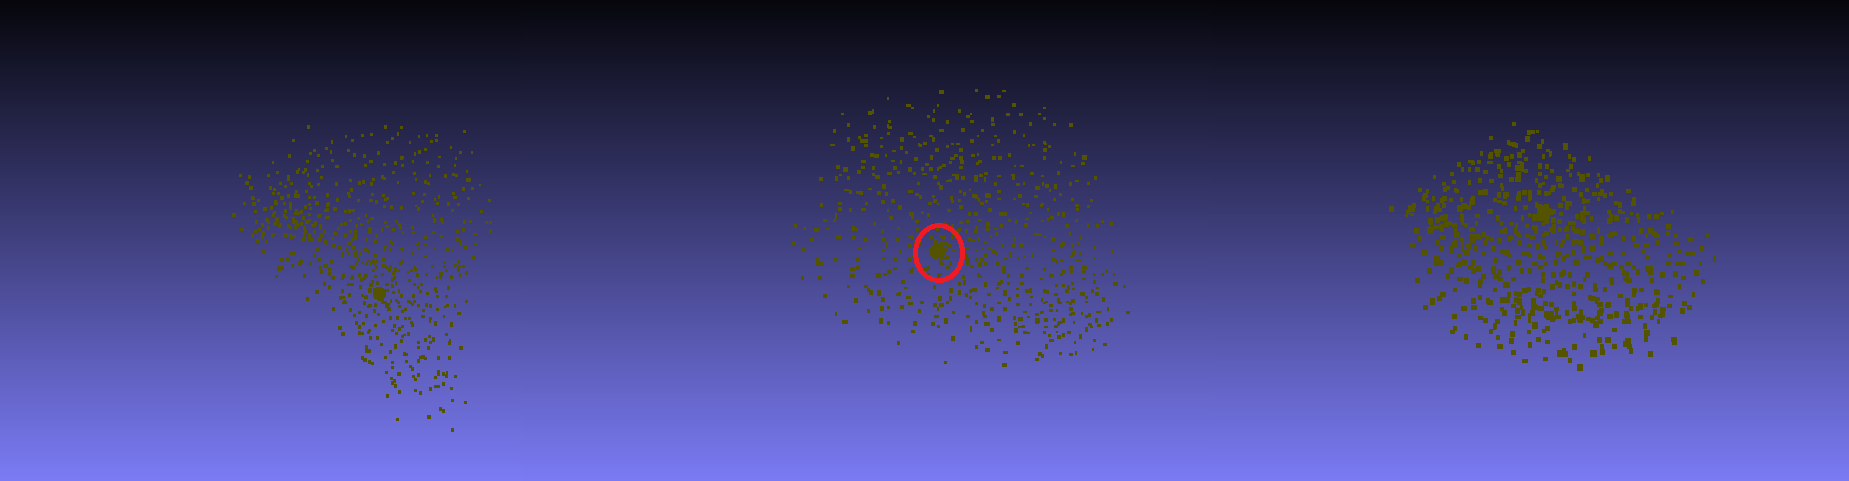
\includegraphics[width=1.0\textwidth]{latent_gan_leaf_example.png}.
	\caption{Trainingsergebnisse des Latent-GAN mit den Blattdaten}
	\label{fig:Bild64}
\end{figure}
\begin{figure}[htbp] 
	\centering
	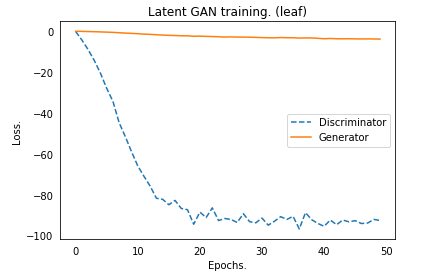
\includegraphics[width=0.6\textwidth]{Latent_gan_training_result.png}
	\caption{Trainingsverlauf des Latent-GAN mit den Blattdaten}
	\label{fig:Bild63}
\end{figure}
\pagebreak\linebreak 
Um die Ergebnisse von Testaufbau „1.2 Latent-GAN mit Stuhldaten“ besser vergleichbar zu machen und um ersichtlich zu machen, ob eine Erhöhung der Anzahl der Tabakblätter-Daten zu einem besseren Ergebnis führen kann und die Punktanhäufung sich reproduzieren lässt, wurden 422 Stuhldaten herangezogen, um das Latent-GAN zu trainieren.  Abb. \ref{fig:Bild66} sind die exemplarisch erzeugten Daten des Generator zu entnehmen. Zu erkennen ist ein ähnliches Phonemen wie bei den Blattdaten. Hohe Punktanhäufungen finden sich an den Kanten der Sitzfläche, zum Übergang der Stuhlbeine. Dadurch lassen sich Rückschlüsse darauf ziehen, dass eine Erhöhung der Daten zu einer besseren Qualität führen kann. Der Trainingsverlauf kann aus Abb. \ref{fig:Bild65} entnommen werden. Auch dieser Verlauf zeigt eine Stagnation schon über mehre Epochen an und verspricht keine Erhöhung der Qualität beim weiteren Verlauf des Trainings.
\begin{figure}[htbp] 
	\centering
	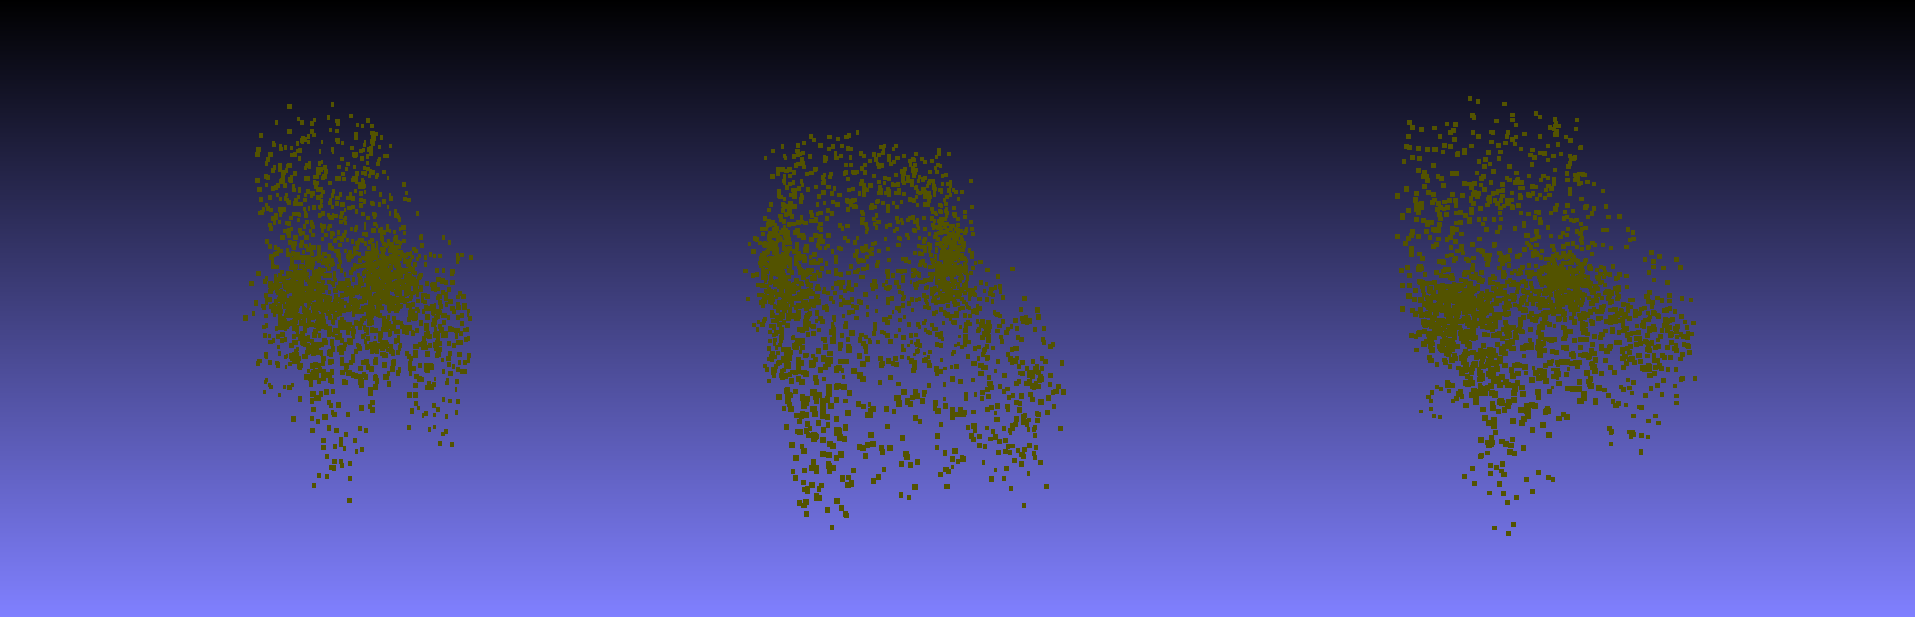
\includegraphics[width=1.0\textwidth]{raw_gan_latent_gan_chair_example_400.png}
	\caption{Trainingsergebnisse des Latent-GAN mit den Stuhldaten und 422 Trainingsdaten}
	\label{fig:Bild66}
\end{figure}
\begin{figure}[htbp] 
	\centering
	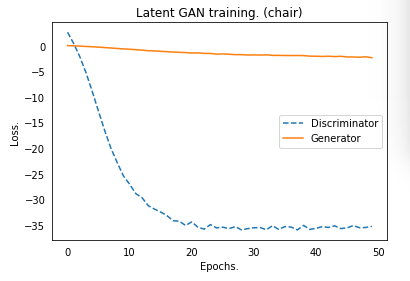
\includegraphics[width=0.6\textwidth]{raw_gan_latent_gan_chair_result_400_example.png}
	\caption{Trainingsverlauf des Latent-GAN mit den Stuhldaten und 422 Trainingsdaten}
	\label{fig:Bild65}
\end{figure}
\pagebreak\linebreak
Zusammengefasst, primär in Hinblick auf den Blattdatensatz, lässt sich feststellen, dass anhand des Stuhldatensatzes die Ergebnisse von Achlioptas, Panos und Diamanti \cite{3dgan} reproduziert werden konnten. Bei einem Datensatz, welcher durch Scanverfahren am Beispiel von Tabakblättern an realen Objekten durchgeführt wurde, konnte gezeigt werden, dass durch das Latent-GAN eine erste Annäherung an qualitativ hochwertig generierte Daten zu sehen ist. Durch eine Erhöhung der Trainingsdaten lässt sich auch eine Steigerung der Qualität feststellen, wie am Beispiel der Stuhldaten durch RAW-GAN und Latent-GAN gezeigt wurde. Es können jedoch keine Aussagen darüber getroffen werden, in welchem Umfang eine Qualitätssteigerung stattfinden kann. 
\\\\
Die Datensätze unterscheiden sich in ihrer Aufbereitung. Die Stuhldaten sind stärker auf einen Koordinatenursprung geeicht, wie auf Abb. \ref{fig:Bild85} festzustellen ist. Auf dieser Abbildung sind mehre Stühle zum Vergleich in ein Koordinatensystem geladen. Abb. \ref{fig:Bild1001} zeigt das gleiche Konzept zum direkten Vergleich anhand von Blattdaten. Zu erkennen ist eine viel höhere Überschneidung der einzelnen Punktwolken aufeinander, als es bei den Blättern der Fall ist. Daraus lässt sich erschließen, dass bei Stühlen gefestigtere Strukturen vorhanden sind und dadurch weniger Varianz bei den Punktwolken untereinander entsteht. Dies hilft dabei, den Suchraum für die GANS einzuschränken und erleichtert das Training am Stuhldatensatz. Bei den Blattdaten müssten bessere Datenvorverarbeitungsschritte erhoben werden, wie beispielsweise ein genaueres Festhalten des Massenzentrums aller Blätter, auf dem Koordinatenursprung.
\\\\ 
Außerdem sind 422 Blattdaten im Vergleich zum Umfang von 6778 Stuhldaten sehr gering und verschlechtern so die Möglichkeit des Latenten-GAN und RAW-GAN, die Grundgesamtheit der Daten abzudecken. Aus technischer Sicht könnten andere Layer Strukturen für bessere Ergebnisse sorgen. Die Bearbeitung mit Convolution-Layern auf Bilddaten hat den  Durchbruch bei der Rekonstruktion von Bilddaten überhaupt erst möglich gemacht\cite{imagerecon}. Da der verwendete Generator nur aus Fully-Connected-Layern besteht und die Komplexität von 3D-Punktwolken höher ist,  als die von Bildern, kann an dieser Stelle noch nachgearbeitet werden. Beispielsweise könnte ein 1D-Deconvolutional-Layer implementiert werden, welcher bei Tensorflow 1.12 als Prototyp zur Verfüg-ung steht. Eine andere Möglichkeit wäre es, auf die Arbeit von Cai, Zhongang  und Yu \cite{3d-conv} zurückzugreifen. Diese postuliert eine Herangehensweise für 3D-Convolutional-Methode, welche auf 3D-Punktwolken arbeitet und eine Invarianz im Euklidischen Raum lernt, mit deren Hilfe das Erlernen von Rotationen der Punktwolken möglich gemacht werden soll.
\begin{figure}[htbp] 
	\centering
	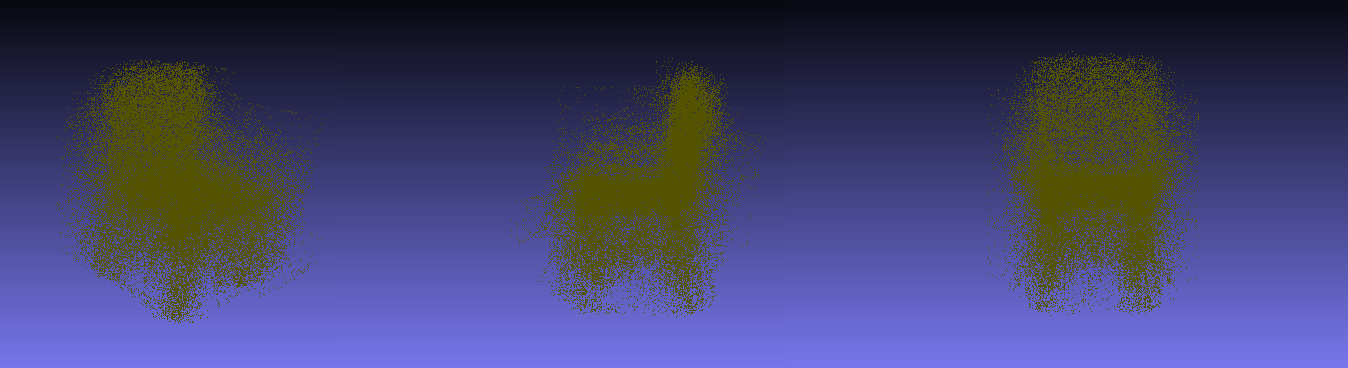
\includegraphics[width=1.0\textwidth]{chair_all.png}
	\caption{24 Stuhldaten in einen Koordinatensystem geladen}
	\label{fig:Bild85}
\end{figure}
\newpage
\subsection{Ergebnisse - Versuchsaufbau 2}

Für Versuchsaufbau 2.1, vgl. \ref{sec:versuch2-aufbau}, wurde zunächst der Autoencoder mit den zerstörten Blattdaten auf 500 Epochen trainiert, um eine komprimierte Version auf 128-D zu erlernen. Dabei wurde zunächst die, in Kapitel \ref{sec:autoencoder} vorgestellte, Chamfer Distanz als Distanzmaß heran genommen. Beispiel Trainingsdatensätze können Abb. \ref{fig:Bild1003} entnommen werden, mit dem jeweils erzeugten Output des Decoders auf Abb. \ref{fig:Bild68}.  
\begin{figure}[htbp] 
	\centering
	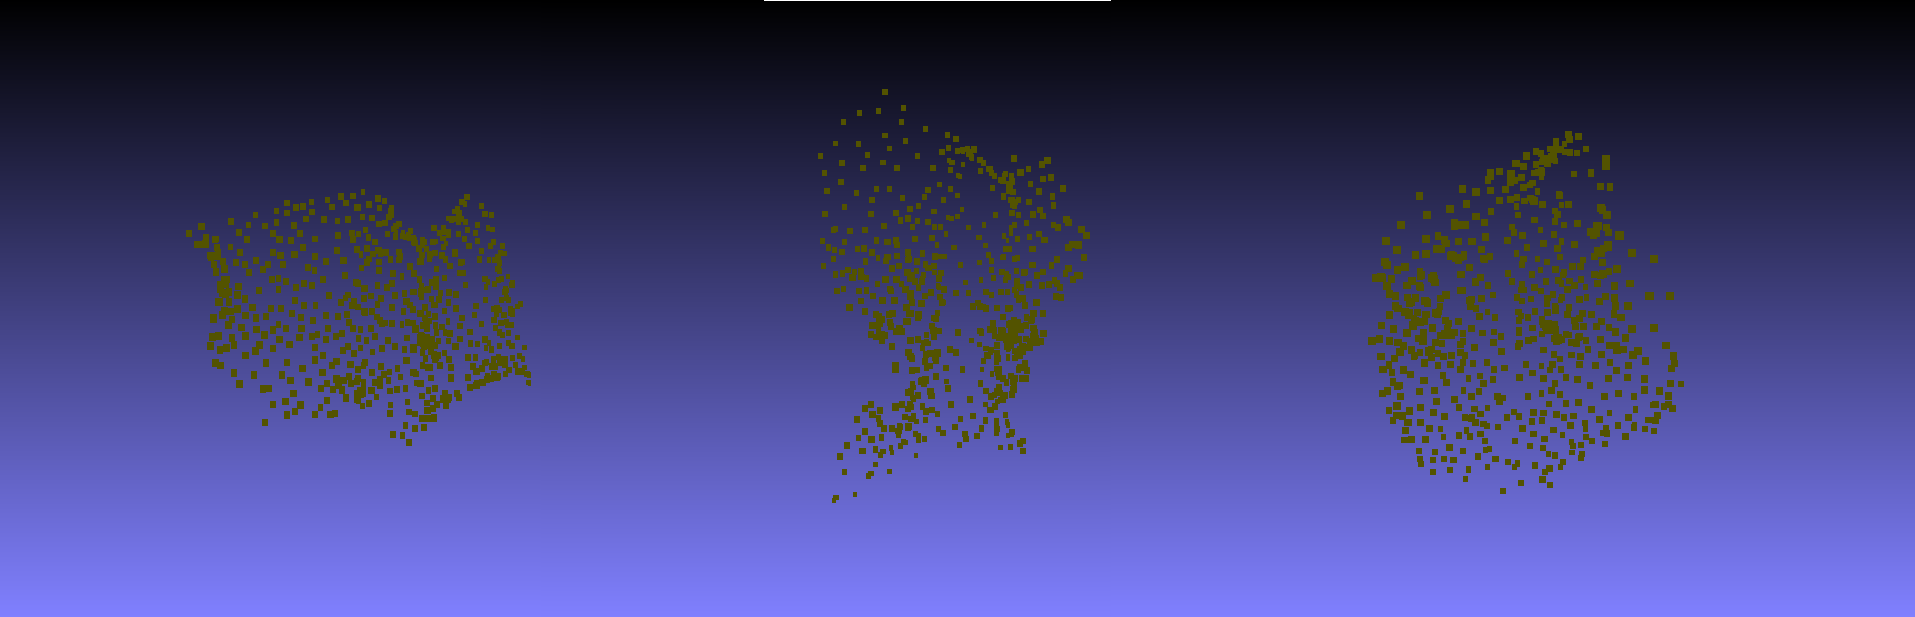
\includegraphics[width=1.0\textwidth]{autoencoder_destroyed_example_chamfer_fake.png}
	\caption{Trainingsbeispiele des Autoencoder mit CD für zerstörte Blattdaten - Output}
	\label{fig:Bild68}
\end{figure}
\begin{figure}[htbp] 
	\centering
	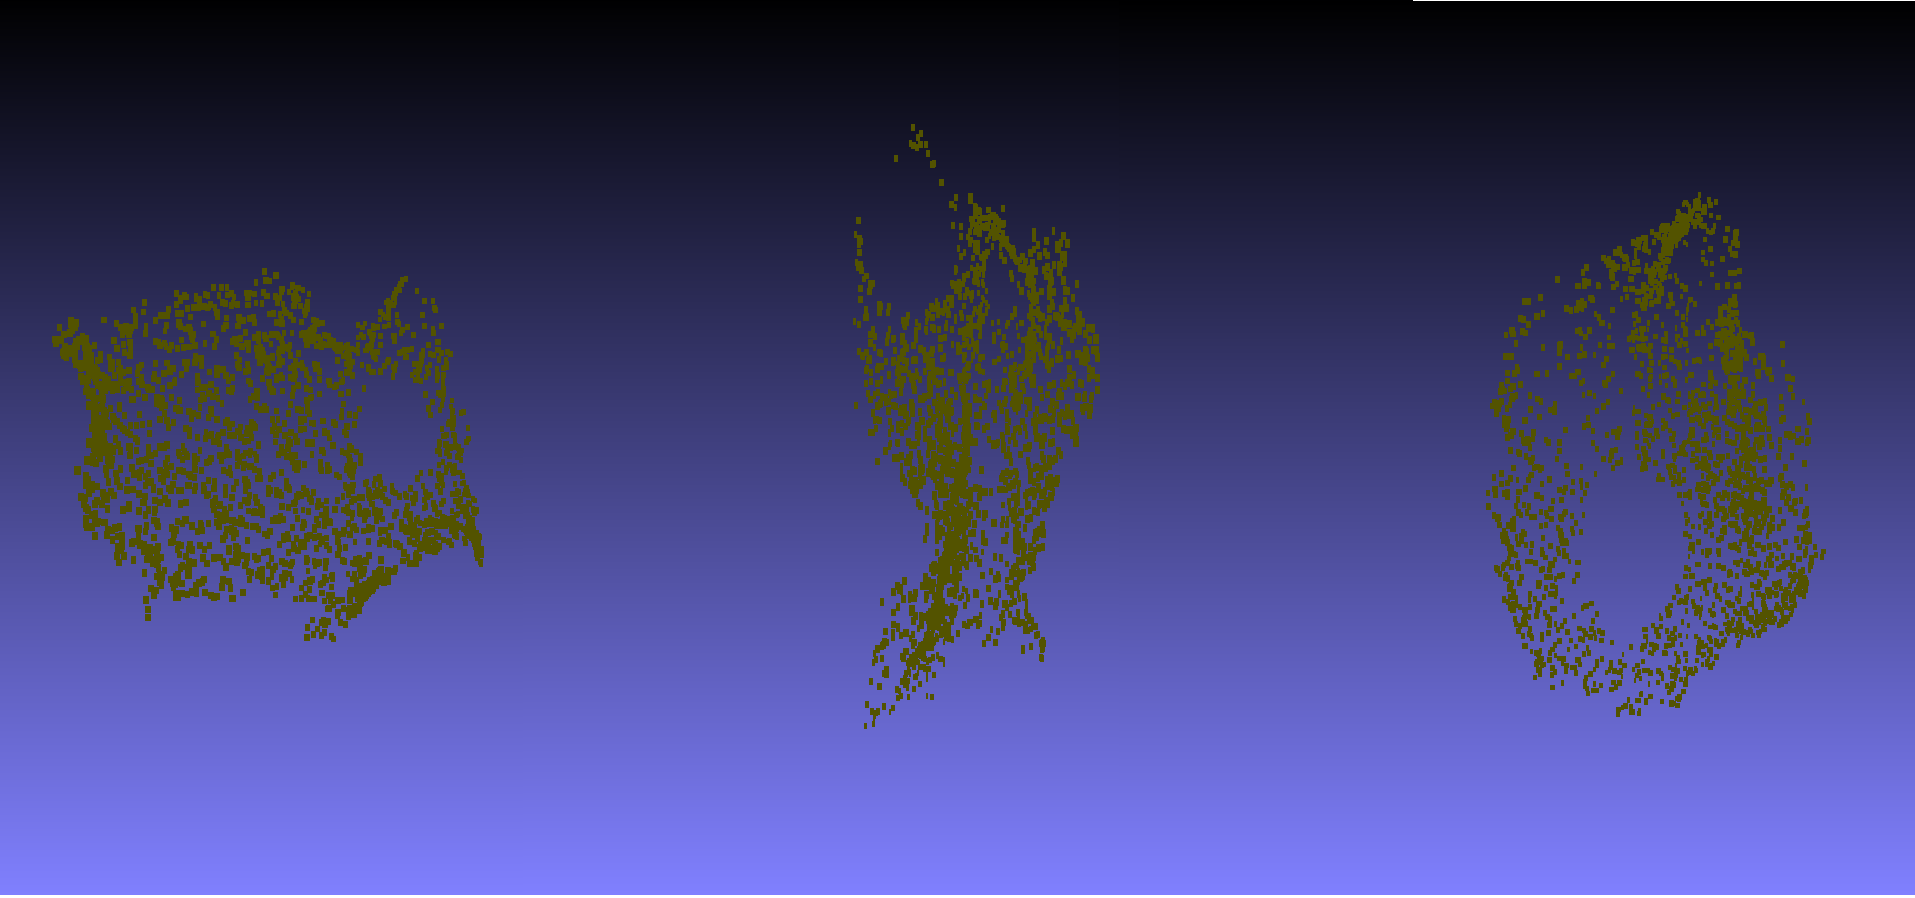
\includegraphics[width=1.0\textwidth]{autoencoder_destroyed_example_chamfer_real.png}
	\caption{Trainingsbeispiele des Autoencoder mit CD für zerstörte Blattdaten - Input}
	\label{fig:Bild1003}
\end{figure}
Wie zu erkennen ist, vervollständigt der Autoencoder mit CD die Blätter selbstständig, obwohl dies nicht als Ziel in diesem Bearbeitungsschritt vorgeben war. Es ist zu erkennen, dass die Dichte, in welcher die Punkte beim Output auf der Höhe der Löcher angeordnet sind, stark von den übrigen Bereichen auf dem Blatt abweicht. 
Auch lässt der Trainingsverlauf in Abb. \ref{fig:Bild67} darauf schließend, dass der Autoencoder selbst beim weiteren Training keine bessere Codierung erlernen wird, welche keine Löcher in den Blättern mehr erzeugt, da das Training  seit Epoche 300 stagniert. Außerdem lässt der durch CD berechnete Abstand zwischen den beiden Punktwolken keine starke Verbesserung mehr zu, da die durchschnittliche Diskrepanz nach dieser Metrik zwischen dem Input x und dem von Decoder erzeugten Output x` nur noch im 0.0005 Bereich liegt, wie auf Abb. \ref{fig:Bild67} nach Epoche 500 abzulesen ist. Da keine verwendbaren Trainingsdaten für den Latenten C-GAN Versuchsaufbau 2.1 generiert werden konnten, soll an dieser Stelle der Versuchsaufbau 2.1 Latent C-GAN  mit Chamfer Distanz nicht weiter geführt werden. 
\begin{figure}[htbp] 
	\centering
	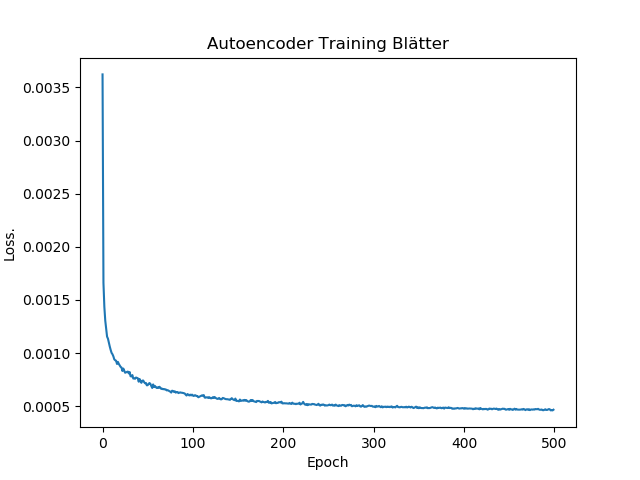
\includegraphics[width=0.6\textwidth]{autoencoder_training_blaetter_result.png}
	\caption{Trainingsverlauf des Autoencoder mit CD für zerstörte Blattdaten}
	\label{fig:Bild67}
\end{figure}
\pagebreak\linebreak 
Um ein bessere Validierungsergebnisse zu erhalten, wurde Versuchsaufbau 2.1 Latent-CGAN ebenfalls mit EMD Zielfunktion für Autoencoder getestet. Es wurden 800 Epochen trainiert. Die Ergebnisse sind ähnlich zu denen mit der CD, vgl. \ref{sec:autoencoder}. Beispiele zum Trainingsinput der Trainingsdatensätze können Abb. \ref{fig:Bild71} entnommen werden mit dem jeweilig erzeugtem Output des Decoders auf Abb. \ref{fig:Bild72} verglichen werden. Wie zu erkennen ist, vervollständigt der Autoencoder mit der EMD die Blattflächen selbstständig, obwohl dies nicht als Ziel des Autoencoder vorgegeben war, sondern lediglich das Erlernen einer Kodierung. Es lässt sich erkennen, dass die Blätter an der Stelle des Loches gleichmäßiger verteilt sind und es keine höheren Punktansammlungen auf der Blattfläche gibt. Wenn man die Ergebnisse mit Hinblick auf die Zielfunktion bewertet, liefert die CD ein besseres Ergebnis. Die Begründung hierfür ist, dass die Punkte auf der Blattoberfläche der Blätter gleichmäßiger verteilt sind. Möchte man nun die beiden Ergebnisse ebenfalls anhand der Qualität des Rekonstruieren beurteilen, obwohl dies nicht das eigentliche Ziel ist, sticht die EMD hervor, da die Punkte im Bereich der Löcher gleichmäßiger verteilt sind.
\begin{figure}[htbp] 
	\centering
	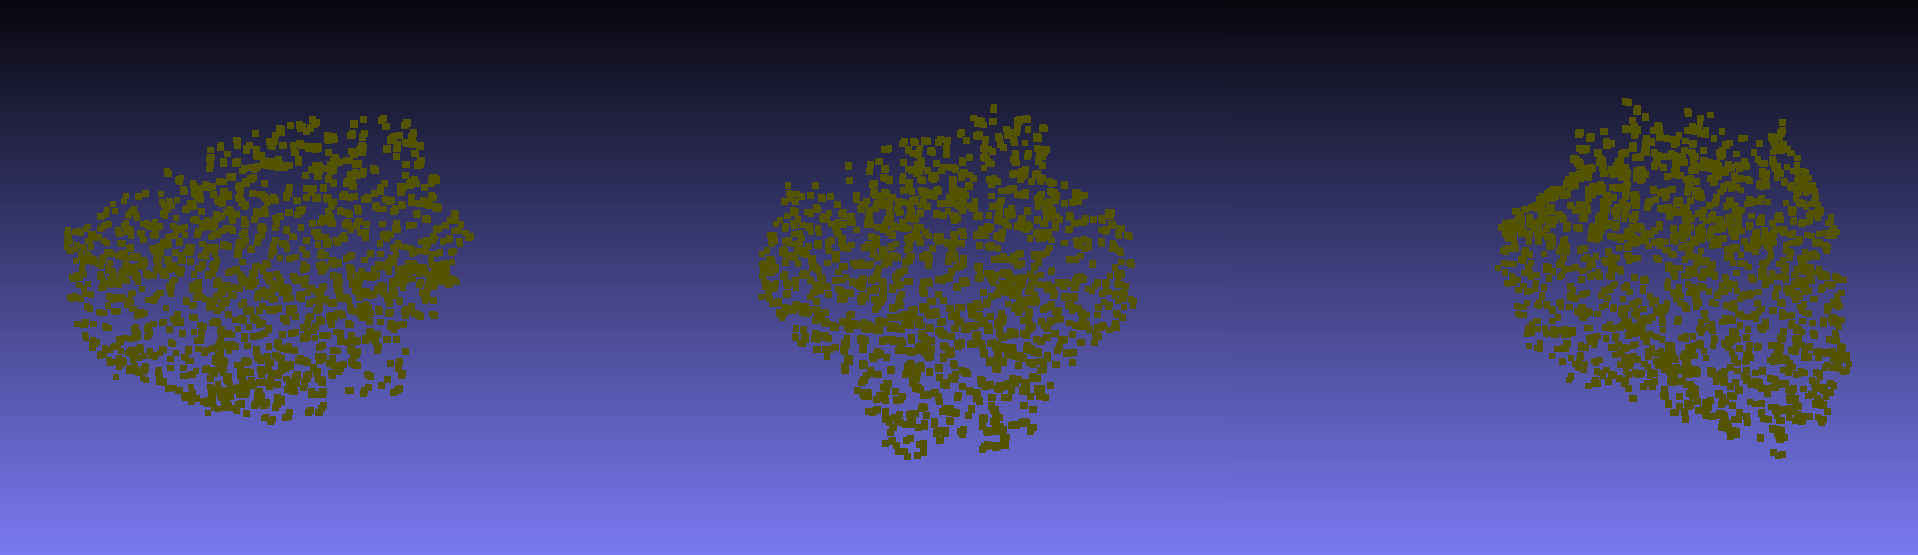
\includegraphics[width=1.0\textwidth]{repairded_emd.png}
	\caption{Trainingsbeispiele des Autoencoder mit EMD für zerstörte Blattdaten - Output}
	\label{fig:Bild72}
\end{figure}
\begin{figure}[htbp] 
	\centering
	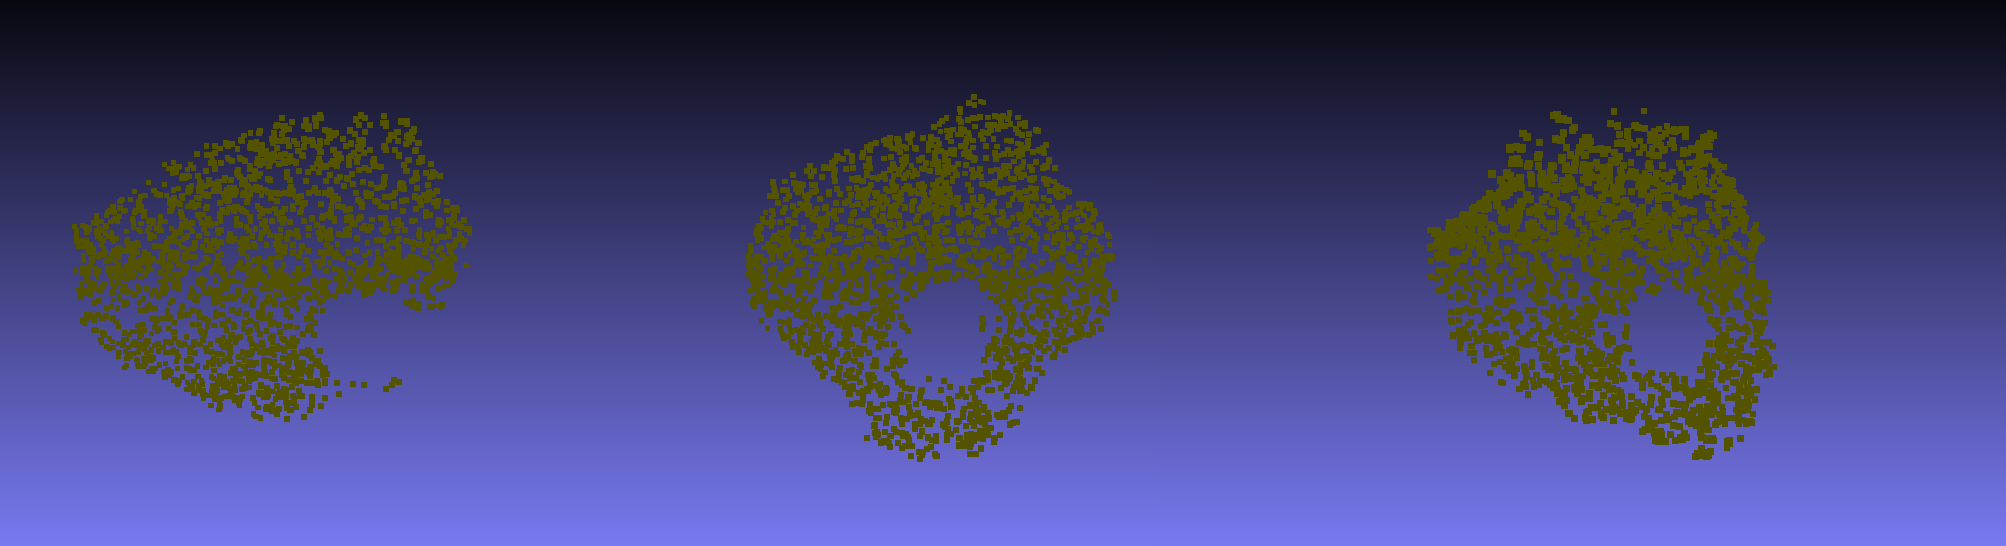
\includegraphics[width=1.0\textwidth]{input_emd.png}
	\caption{Trainingsbeispiele des Autoencoder mit EMD für zerstörte Blattdaten - Input}
	\label{fig:Bild69}
\end{figure}
\\\\
Insgesamt lässt sich feststellen, dass die Distanzen niedriger sind und die Dichte der Löcher abnimmt. Jedoch liefert die EMD den positiven Nebeneffekt, dass die Blätter realistischer rekonstruiert werden. Da das Training seit Epoche 300 stagniert, ist darauf zu schließend, dass selbst beim weiteren Training keine Löcher, welche in den Blättern entstehen sollen, herzustellen sind. Außerdem lässt der, durch die Chamfer Distanz berechnete, Abstand zwischen den beiden Punktwolken keine starke Verbesserung mehr zu, da die durchschnittliche Diskrepanz zwischen dem Input x und den vom Decoder erzeugten Output x`, nur noch im 0.03 Bereich liegt. Dies ist auf Abb. \ref{fig:Bild67} in Epoche 500 abzulesen. Das Training entwickelt sich jedoch seit mehreren Epochen nicht weiter und stagniert. Auch mit dieser Anwendung kann das Latente C-GAN demzufolge nicht weitergeführt werden, da keine erfolgreichen Trainingsdaten erzeugt werden konnten.
\begin{figure}[htbp] 
	\centering
	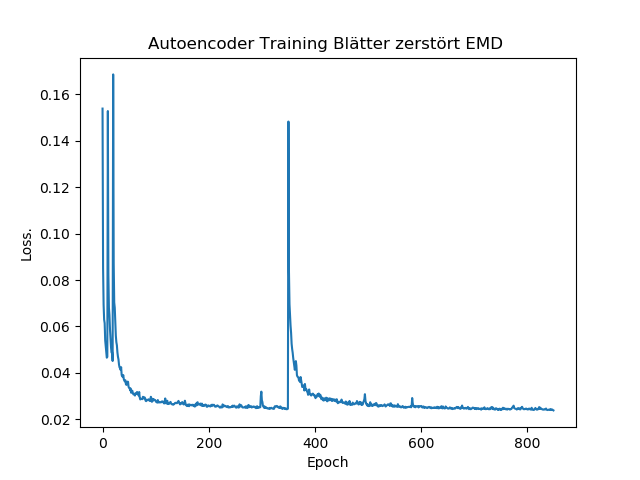
\includegraphics[width=0.7\textwidth]{autoencoder_training_bleatter_zer_result_emd.png}
	\caption{Trainingsverlauf des Autoencoder mit EMD für zerstörte Blattdaten }
	\label{fig:Bild71}
\end{figure}
\newpage
~\\\\
Für den Versuchsaufbau 2.2 RAW-CGAN mit Fully-Connected-Layern mit EMD ist auf Abb. \ref{fig:Bild75} rechts der Loss des Discriminators abgebildet und links der Loss des Generators. Der Loss des Generator sinkt zwar, jedoch ähneln die generierten Trainingsbeispiele in Abb. \ref{fig:Bild77} keinen reparierten Blätter. Der dazugehörige Input ist auf Abb.\ref{fig:Bild76} zu sehen. Da der Generator bereits an sein Limit gerät und keine erheblichen Verbesserungen mehr möglich sind, ist festzustellen, dass durch einen Generator mit Fully-Connected-Layern keine Blattdatenrekonstruktion stattfinden kann.   
\begin{figure}[htbp] 
	\centering
	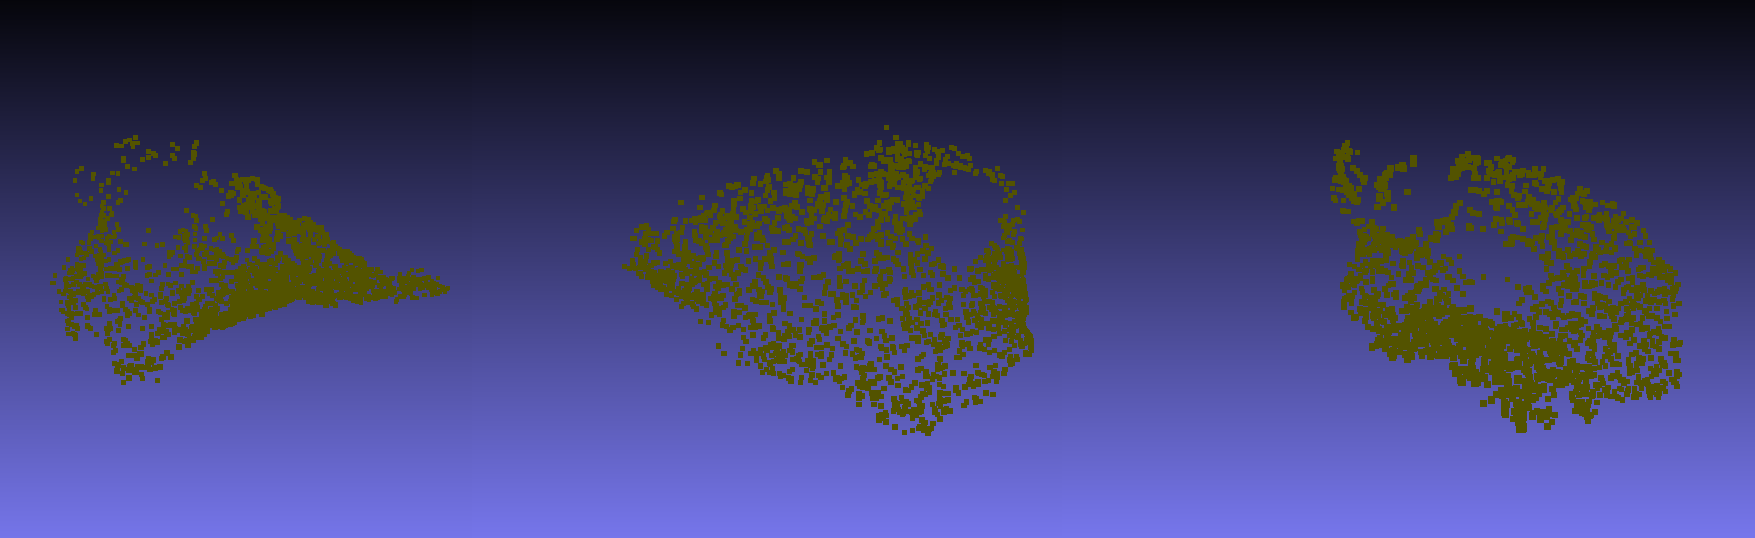
\includegraphics[width=1.0\textwidth]{reaf_fully_connected_wgan_.png}
	\caption{Der Input aus welchen vom RAW-CGAN mit EMD die Daten rekonstruiert wurden}
	\label{fig:Bild76}
\end{figure}
\begin{figure}[htbp] 
	\centering
	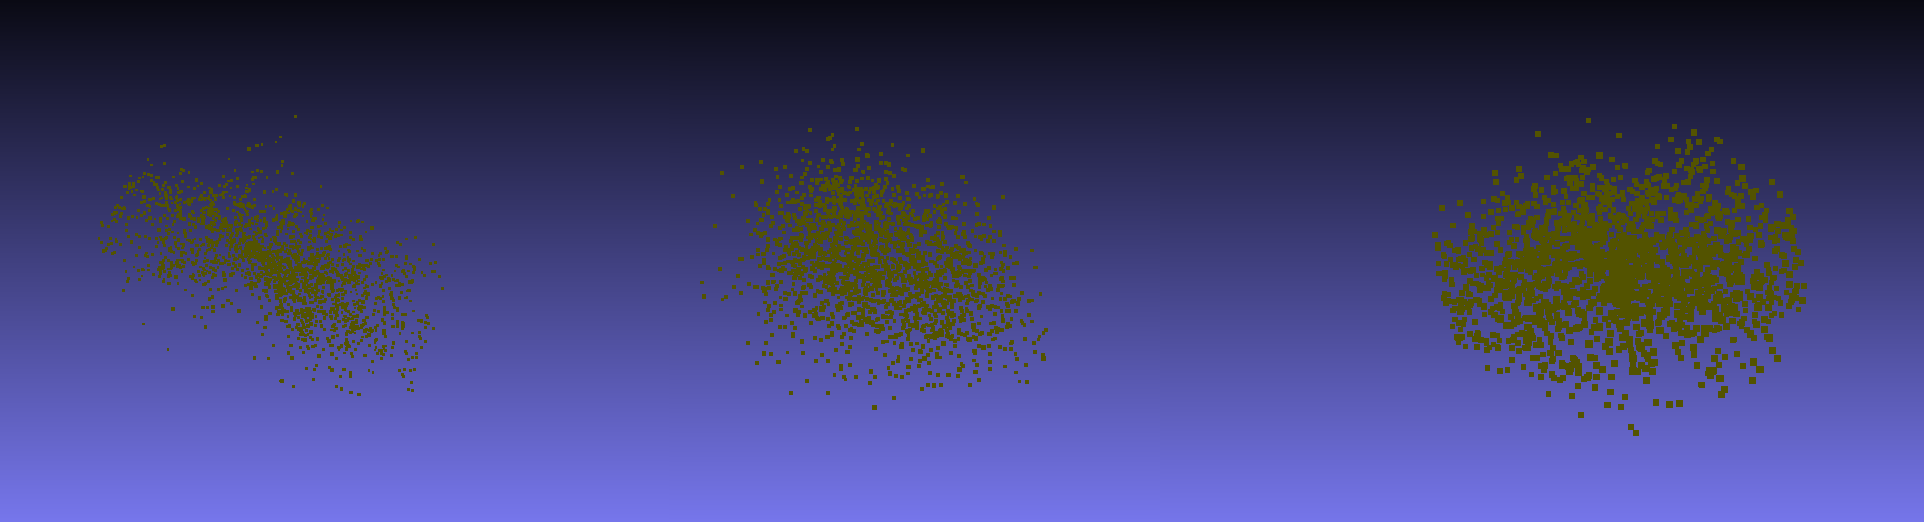
\includegraphics[width=1.0\textwidth]{fake_wgan_fully_rawcgan.png}
	\caption{Output des Generators vom RAW-CGAN mit EMD}
	\label{fig:Bild77}
\end{figure}
\begin{figure}[htbp] 
	\centering
	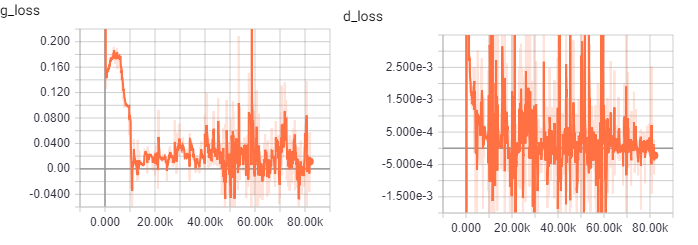
\includegraphics[width=0.8\textwidth]{wasserstein_fully_connected_rawcgan_loss.png}
	\caption{Generator und Discriminator Loss des RAW-CGAN mit EMD}
	\label{fig:Bild75}
\end{figure}
\newpage
~\\\\
In Folgenden werden die Ergebnisse von Testaufbau 2.2 RAW-CGAN mit Con-volutional-Layer im Discriminator und der Vanilla-GAN-Loss vorgestellt. Der Trainingsverlauf von Generator und Discriminator kann Abb. \ref{fig:Bild79} entnommen werden. Die Sprünge wirken auf den ersten Blick sehr stark, beachtet man jedoch die Skalenwert auf der Y-Achse des Generators, bewegt sich der Loss zwischen 0.691 und 0,696. Dies lässt auf keine starke Verbesserung schließen. Der Discriminator kann die Unterscheidung von Fake und Real Datensatz perfekt erkennen. Das Training läuft über mehre Epoche konstant hinweg und lässt auch für einen längeren Durchlauf auf keine Verbesserung schließen. Einige Beispieltabakblätter, welche vom Generator erstellt wurden,  können aus Abb. \ref{fig:Bild80} entnommen werden, so wie der dazu gehörige Input aus Abb. \ref{fig:Bild78}. Darauf sind jedoch keine hohen Ähnlichkeiten zu Blättern zu erkennen. Verglichen mit RAW-CGAN mit Fully-Connected-Layern ist eine Verbesserung festzustellen, da sich bessere Blattränder abbilden. Jedoch führen starke Punktansammlungen nicht zu dichten Blattflächen. Da nach der Loss Funktion keine gravierenden Veränderungen mehr zu erwarten sind, kann festgehalten werden, dass keine Rekonstruktion von zerstörten Blattdaten mit dem in Kapitel \ref{sec:versuch2-aufbau} beschriebenen RAW-CGAN mit Convolutional-Layer und Vanilla-GAN-Loss möglich ist.
\begin{figure}[htbp] 
	\centering
	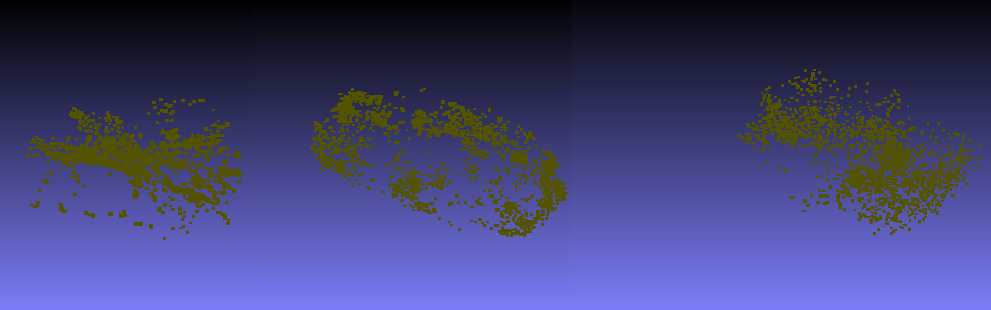
\includegraphics[width=1.0\textwidth]{dcpgan_ws_fake.png}
	\caption{Der Output, aus welchen vom RAW-CGAN mit Convolutional Layern die Daten rekonstruiert wurde}
	\label{fig:Bild80}
\end{figure}
\begin{figure}[htbp] 
	\centering
	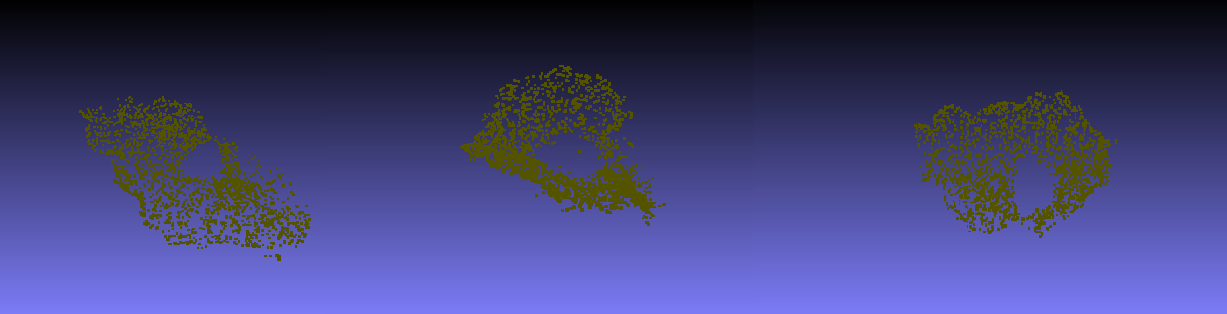
\includegraphics[width=1.0\textwidth]{dc_pgan_ws_real.png}
	\caption{Der Input, aus welchen vom RAW-CGAN mit Convolutional Layern die Daten rekonstruiert wurden}
	\label{fig:Bild78}
\end{figure}
\begin{figure}[htbp] 
	\centering
	\includegraphics[width=1.0\textwidth]{cgan_loss_vanilla.png}
	\caption{RAW-CGAN mit Convolutional-Layern und Vanilla-GAN-Loss}
	\label{fig:Bild79}
\end{figure}
\newpage
~\\\\
Zuletzt werden die Ergebnisse von Testaufbau 2.2 RAW-CGAN mit Deconvo-lutional-Layer mit der Wasserstein-Metrik vorgestellt, die mit den nicht komprimierten Daten trainiert wird.  Der Trainingsverlauf von Generator und Discriminator kann Abb. \ref{fig:Bild1001} entnommen werden.  Der Verlauf des Discriminator Loss arbeitet sich konstant nach unten und hat zwei Ausbrecher, welche aber kein Einfluss auf den weiteren Trainingsverlauf haben, da der Generator durch den Gradienten keinen Aufschwung erlangt. Der Generator springt zwar am Ende des Trainings noch, jedoch sind die Sprünge in einem so niedrigen Intervall, dass keine große Veränderung mehr zu erwarten sind. Die vom Generator generierten Outputs auf Abb. \ref{fig:Bild82} und deren dazugehöriger Input auf Abb. \ref{fig:Bild83} zeigen bereits die Umrisse der Blätter auf, jedoch sind die Blattflächen nicht gebildet. 
\begin{figure}[htbp] 
	\centering
	\includegraphics[width=1.0\textwidth]{cgan_ws_loss.png}
	\caption{Discriminator und Generator Loss RAW-DGAN mit Convolutional-Layer und Wasserstein Metrik}
	\label{fig:Bild1001}
\end{figure}
\begin{figure}[htbp] 
	\centering
	\includegraphics[width=1.0\textwidth]{raw_cgan_ws_fake.png}
	\caption{Der Output aus welchen vom RAW-CGAN mit Convolutional Layern die Daten rekonstruiert wurde}
	\label{fig:Bild82}
\end{figure}
\begin{figure}[htbp] 
	\centering
	\includegraphics[width=1.0\textwidth]{raw_cgan_ws_real.png}
	\caption{Der Input aus welchen vom RAW-CGAN mit Convolutional Layern die Daten rekonstruiert wurden}
	\label{fig:Bild83}
\end{figure}
Fasst man Versuchsaufbau 2 zusammen, ist festzustellen, dass in Versuchsaufbau 2.1 abgebrochen werden musste, da die Autoencoder nicht fähig waren, die zerstörten Trainingsdaten zu erlernen. Jedoch konnten sie die Daten rekonstruieren, obwohl dies nicht als Ziel für die Autoencoder definiert war. Ob eine praktische Anwendung hierdurch ermöglicht ist und ob diese Rekonstruktion nur für die Form von Blättern möglich ist, oder beispielsweise auch ähnliche Ergebnisse beim Stuhldatensatz erlangt werden können, muss in zukünftigen Arbeiten geprüft werden.
\\\\
Im Versuchsaufbau 2.2 zeigen sich mit der Verwendung von Convolutional-Layer im Discriminator bessere Ergebnisse. Ein qualitativer Unterschied zwischen dem Versuchsaufbau 2.2 RAW-CGAN mit Convolutional-Layer und Vanilla-GAN oder Wasserstein Metrik lässt sich nicht feststellen. Jedoch lässt die Convolutional-Layer das Erlernen der Latenten-Struktur besser gelingen. Eine Rekonstruktion ist aber auch mit diesem Model nicht möglich. Jedoch kann nicht ausgeschlossen werden, dass GAN durch andere Aufbauten, wie beispielsweise mit 1D-Deconvolutional-Layer, implementiert werden, welche bei Tensorflow 1.12 als Prototyp zur Verfügung steht. Eine weitere Möglichkeit wäre es, auf die Arbeit von Cai, Zhongang  und Yu \cite{3d-conv} aufzubauen. Diese postuliert eine Herangehensweise für 3D-Convolutional- Methode, welche auf 3D-Punktwolken arbeitet und eine Invarianz im Euklidischen Raum lernt, mit deren Hilfe es möglich sein soll, Rotationen der Punktwolke zu erlernen. Durch diese neuen Module könnte das Erlernen des latenten Raumes von 3D-Punktwolken möglich gemacht werden und das letztendliche Ziel, 3D-Punktwolken zu rekonstruieren, erreicht werden.   
\begin{figure}[htbp] 
	\centering
	\includegraphics[width=1.0\textwidth]{problem_autoencoder.png}
	\caption{Rot der Output des Autoencoders in Epoche 1, Grün der Input des Autoencoders }
	\label{fig:Bild1005}
\end{figure}
Im Versuchsaufbau 2.2 zeigen sich mit der Verwendung von Convolutional-Layer im Discriminator bessere Ergebnisse. Ein qualitativer Unterschied zwischen dem Versuchsaufbau 2.2 RAW-CGAN mit Convolutional-Layer und Vanilla-GAN oder Wasserstein Metrik lässt sich nicht feststellen. Jedoch lässt die Convolutional-Layer das erlernen der Latenten-Struktur besser gelingen. Eine Rekonstruktion ist aber auch mit diesen Model nicht möglich. Jedoch kann nicht ausgeschlossen sein das GAN durch andere Aufbauten wie Beispielsweise mit 1D-Deconvolutional-Layer, implementiert werden, welche bei Tensorflow 1.12 als Prototyp zur Verfügung steht. Eine weitere Möglichkeit wäre auf die Arbeit von Cai, Zhongang  und Yu \cite{3d-conv} anzusetzen dieser postuliert eine Herangehensweise für 3D-Convolutional- Methode, welche auf 3D-Punktwolken arbeitet und eine Invarianz im Euklidischen Raum lernt mit deren Hilfe es möglich sein soll Rotationen der Punktwolke zu erlernen. Durch diese neuen Module könnte das Erlernen des latenten Raumes von 3D-Punktwolken möglich gemacht werden und das letztendliche Ziel, 3D-Punktwolken zu rekonstruieren erreicht werden. 
\newpage
\section{Zusammenfassung und Diskussion }

Verglichen mit anderen Daten, wie Bildern oder Audio, bleiben 3D-Daten eine Herausforderung, da ihr Suchraum erheblich höher ist, wie auch in Kapitel \ref{sec:3dprobleme} thematisiert. Durch den Informationsgehalt von Punktwolken erhöht sich der Suchraum für GANs und stellt Forscher vor neue Herausforderungen. Die Fragestellungen, welchen in dieser Arbeit nachgegangen werden sollte, lauten:
\begin{description}
\item[Fragestellung 1] Können durch GANs 3D-Punktwolken von Tabakblättern erlernt werden um neue Datensätze zu generieren?\\
\item[Fragestellung 2] Können durch GANs 3D-Punktwolken von Tabakblättern, die von ihrem Urzustand abgebracht wurden, rekonstruiert werden? 
\end{description}
Es konnte festgestellt werden, dass die Fragestellung 1 (vgl. \ref{sec:versuch1-aufbau}) positiv beantwortet werden kann, jedoch noch Verbesserungen, in der Qualität der durch GANs generierten 3D-Punktwolken, möglich sind. Der Aufbau, welcher derzeit die besten Ergebnisse hervorbringt, ist das Latent-GAN. Aber auch beim RAW-GAN für Punktwolken ist eine Erhöhung der Qualität festzustellen, wenn mehr Daten zur Verfügung stehen. Außerdem könnte eine systematischere Datenvorverarbeitung der Trainingsdaten bessere Ergebnisse hervorbringen, wie beispielsweise eine Zentrierung der Massepunkte jedes Blattes auf den Koordinatenursprung, oder eine einheitlichere Ausrichtung der Blattflächen zu einem Fixpunkt im Euklidischen Raum. Beim strukturellen Aufbau des GAN könnte ein 1D-Deconvolutional-Layer implementiert werden, welche bei Tensorflow 1.12 als Prototyp zur Verfügung steht. Eine andere Möglichkeit wäre es, auf die Arbeit von Cai, Zhongang  und Yu \cite{3d-conv} zurückzugreifen. Diese postuliert eine Herangehensweise für 3D-Convolution Methode, welche auf 3D-Punktwolken arbeitet und eine Invarianz im Euklidischen Raum lernt, mit deren Hilfe das Erlernen von Rotationen der Punktwolken möglich gemacht werden soll.
\\\\
Zu Fragestellung 2, welche in Kapitel \ref{sec:versuch2-aufbau} überprüft wurde, ist festzuhalten, dass der Aufbau des Latent-CGAN abgebrochen werden musste, da der Autoencoder die zerstörten Trainingsdaten nicht erlernen konnte und somit eine weitere Durchführung des Versuchsaufbaus unmöglich machte. Jedoch war festzustellen, dass die Autoencoder die Löcher in den Blättern mit Punkten füllten und somit eine Rekonstruktion möglich machten. Dies ist auf die beiden Zielfunktionen des Autoencoder zurückzuführen, welche durch das Distanzmaß zwischen 2 Punktwolken dafür sorgt, dass die Punktwolken gedehnt werden. Ob dadurch eine praktische Anwendung möglich ist und ob diese Rekonstruktion nur für die Form von Blättern gilt, oder beispielsweise auch ähnliche Ergebnisse beim Stuhl Datensatz möglich sind, muss in zukünftigen Arbeiten geprüft werden. Dies kann durch die gleiche Datenverarbeitung, mit den Sphären für Stuhldaten, überprüft werden 
\pagebreak\linebreak 
Das RAW-CGAN zeigte bessere Ergebnisse mit der Verwendung von Convolutio-nal-Layern im Discriminator. Jedoch war auch mit diesem Versuchsaufbau die Rekonstruktion von Daten nicht möglich. Es zeigte sich jedoch eine Verbesserung mit den Convolutional-Layern, im Vergleich zu den Fully-Connected-Layern. Erst durch den Einsatz verbesserter Convolution Methoden wurde die Rekonstruktion und Veränderung von Bildern ermöglicht  \cite{imagerecon} und diese Convolution speziell auf 2D-Daten entwickelt. Daher lässt sich nicht ausschließen, dass durch die Verwendung von Layern, welche speziell für 3D-Daten entwickelt werden, bessere Ergebnisse hervorgebracht werden können. Auch hier kann, wie bei Fragestellung 2, beispielsweise mit 1D-Deconvolutional-Layer implementiert werden. Eine andere Möglichkeit wäre es, auf der Arbeit von Cai, Zhongang  und Yu \cite{3d-conv} aufzubauen. Diese postulieren eine Herangehensweise für die 3D-Convolution Methode, welche auf 3D-Punktwolken arbeitet und eine Invarianz im Euklidischen Raum lernt, mit deren Hilfe es einfach sein soll, Rotationen der Punktwolke zu erlernen. Durch diese neuen Module könnte das Erlernen des latenten Raumes von 3D-Punktwolken möglich gemacht werden und das letztendliche Ziel, 3D-Punktwolken zu rekonstruieren, erreicht werden.  Eine weitere Möglichkeit ist es auch, die Zielfunktion von GAN zu ändern, wie in der Arbeit von Zhu, Jun-Yan und Park \cite{pix2pix}, in Form ihres Pix2Pix Models. In diesem verwenden sie die C-GAN Loss Funktion und ändern jene, um zusätzlich zur üblichen Loss-Funktion auch die Differenz zwischen Generator Output und dem dazugehörigen Urzustand des Trainingsdatensatz zu berechnen und addieren dies zur Loss-Funktion. Dieses Verfahren könnte auch für Punktwolken übernommen werden und mit der CD oder EMD implementiert werden. Obwohl die qualitative Rekonstruktion von Punktwolken von Tabakblättern nicht zufriedenstellend erreicht werden konnte, besteht dennoch Potential, die in der vorliegenden Abhandlung thematisierten Forschungsfragen in zukünftigen Arbeiten weiter zu verfolgen.
\newpage
\listoffigures
\newpage
\section*{Abkürzungsverzeichnis}
\addcontentsline{toc}{section}{Abkürzungsverzeichnis}
\begin{acronym}[Bash]
	\acro{Abb.} Abbildung
	\acro{C-GAN} Conditional Adversarial Networks
	\acro{CD} Chamfer Distance
	\acro{EMD} Earth Mover Distance
	\acro{KNN} Künstliches Neuronales Netzwerk
	\acro{GAN} Generativ Adverserial Network
	\acro{DC GAN} Deep Convolution Generative Adverserial Network
	\acro{CNN} Convolutional Neural Network
	\acro{KL} Kulback-Leibler Divergenz
	\acro{3D} 3 Dimensional 
\end{acronym}
\newpage
\bibliographystyle{apacite}
\bibliography{mybib}
~\\\\
\pagebreak\linebreak 
\textbf{\large{Verfassererklärung}}\\\\
Ich erkläre hiermit gemäß § 17 Abs. 2 APO, dass ich die vorstehende Masterarbeit
selbstständig verfasst und keine anderen als die angegebenen Quellen und
Hilfsmittel benutzt habe.\\\\\\\\\
\vspace{5.0cm}
\begin{tabular}{lp{2em}l}
	\hspace{3cm}   && \hspace{3cm} \\\cline{1-1}\cline{3-3}
	Datum     && Unterschrift
\end{tabular}
\end{document}
